% use PDFLaTex
%!TEX root = ../document.tex
\documentclass[article,11pt,DIV=8,listof=totoc, lststotoc]{scrreprt}
\usepackage{scrhack}
\usepackage[utf8]{inputenc}
\usepackage[ngerman]{babel}
\usepackage{setspace}
\usepackage{microtype}
\usepackage[T1]{fontenc}
\usepackage[usenames,dvipsnames,svgnames,table]{xcolor}
\usepackage{blindtext}
\usepackage{amsmath}
\usepackage{mathpazo}
\usepackage{FiraSans}
\usepackage[scaled=.98,sups,osf]{XCharter}
\usepackage[scaled=1.04,varqu,varl]{inconsolata}
\usepackage{graphicx}
\usepackage{url}
\usepackage{csquotes}
\usepackage{tikz}
\usepackage{xparse}
\usepackage{listings}
\usepackage{float}
\usepackage{wrapfig}
\setlength{\emergencystretch}{0.5em}
%%%%%%%%%%%%%%%%%%%%%%%%%%%%%%%%%%%%%%%%%%%%%%%%d%%


%%%%%%%%%%%%%%%%%%%%%%%%%%%%%%%%%%%%%%%%%%%%%%%%%%
% colors
\definecolor{THI-Blue}{RGB}{1,90,156}
\definecolor{altgray}{RGB}{240, 240, 240}
\colorlet{BLACK}{black}
\colorlet{documentColor}{THI-Blue}
%%%%%%%%%%%%%%%%%%%%%%%%%%%%%%%%%%%%%%%%%%%%%%%%%%


%%%%%%%%%%%%%%%%%%%%%%%%%%%%%%%%%%%%%%%%%%%%%%%%%%
% listings
\definecolor{darkgreen}{rgb}{0, 0.4, 0}
\lstset{
         basicstyle=\footnotesize\ttfamily, % Standardschrift
         numbers=left,               % Ort der Zeilennummern
         numbersep=5pt,              % Abstand der Nummern zum Text
         tabsize=2,                  % Groesse von Tabs
         extendedchars=true,         %
         breaklines=true,            % Zeilen werden Umgebrochen
         keywordstyle=\color{red},
    		frame=b,         
         stringstyle=\color{blue}\ttfamily, % Farbe der String
         showspaces=false,           % Leerzeichen anzeigen ?
         showtabs=false,             % Tabs anzeigen ?
         xleftmargin=17pt,
         framexleftmargin=17pt,
         framexrightmargin=5pt,
         framexbottommargin=4pt,
         %backgroundcolor=\color{lightgray},
         showstringspaces=false,      % Leerzeichen in Strings anzeigen ?        
         commentstyle=\color{darkgreen}
}
%\lstset{basicstyle=\footnotesize\ttfamily,breaklines=true}
%\lstset{stringstyle=\color{red}} % typewriter type for strings
%\lstset{keywordstyle=\color{blue}\bfseries} \lstset{commentstyle=\color{green}}

\lstloadlanguages{C}


\lstset{literate=%
  {Ö}{{\"O}}1
  {Ä}{{\"A}}1
  {Ü}{{\"U}}1
  {ß}{{\ss}}2
  {ü}{{\"u}}1
  {ä}{{\"a}}1
  {ö}{{\"o}}1
}
%%%%%%%%%%%%%%%%%%%%%%%%%%%%%%%%%%%%%%%%%%%%%%%%%%


%%%%%%%%%%%%%%%%%%%%%%%%%%%%%%%%%%%%%%%%%%%%%%%%%%
% Section font settings
\addtokomafont{chapter}{\leavevmode\color{documentColor}}
\addtokomafont{section}{\leavevmode\color{documentColor}}
\addtokomafont{subsection}{\leavevmode\color{black!70}}
\addtokomafont{title}{\mdseries\Huge\leavevmode\color{documentColor}}
\addtokomafont{author}{\sffamily\color{black!70}}
\addtokomafont{date}{\sffamily\color{black!70}}
\addtokomafont{subtitle}{\Large}
\addtokomafont{subject}{\sffamily\mdseries\color{black!70}\lsstyle}
\addtokomafont{disposition}{\mdseries}
\addtokomafont{paragraph}{\normalfont\bfseries\color{black!80}}
\addtokomafont{caption}{\small\sffamily\color{black!80}}
\addtokomafont{captionlabel}{\sffamily\color{documentColor}}
\setcounter{secnumdepth}{3}
%%%%%%%%%%%%%%%%%%%%%%%%%%%%%%%%%%%%%%%%%%%%%%%%%%


%%%%%%%%%%%%%%%%%%%%%%%%%%%%%%%%%%%%%%%%%%%%%%%%%%
% begin of the document
\usepackage{eso-pic}
\AtBeginDocument{
\newcommand\BackgroundPic{%
 \put(-1,-1){%
\parbox[b][\paperheight]{\paperwidth}{%
\vfill

\includegraphics[width=0.95\paperwidth]{imports/thi_green.png}
\hfill
}
}
\put(0,-120){%
\parbox[b][\paperheight]{\paperwidth}{%
\vfill
\centering

\includegraphics[width=7cm]{imports/thi_logo.pdf}
\\[0.5cm]
\vfill
}}
}
\AddToShipoutPicture*{\BackgroundPic}
\maketitle
\clearpage
}
%%%%%%%%%%%%%%%%%%%%%%%%%%%%%%%%%%%%%%%%%%%%%%%%%%


%%%%%%%%%%%%%%%%%%%%%%%%%%%%%%%%%%%%%%%%%%%%%%%%%%
% Header
\usepackage[automark]{scrlayer-scrpage}
% \pagestyle{headings}
\addtokomafont{pageheadfoot}{\normalfont\small\color{black!60}\sffamily}
\addtokomafont{pagefoot}{\small}
\addtokomafont{pagehead}{\small}
\addtokomafont{pagenumber}{\normalfont\small\color{black!60}\sffamily}
\newcommand\spacedlowsmallcaps[1]{\scshape\lsstyle \MakeLowercase{#1}}
\newcommand\spacedallcaps[1]{#1}

\clearscrheadings
%\renewcommand{\sectionmark}[1]{\markright{\thesection\enspace\spacedlowsmallcaps{#1}}}
\renewcommand{\chaptermark}[1]{\markboth{\spacedlowsmallcaps{#1}}{\spacedlowsmallcaps{#1}}}
\lehead{\mbox{\llap{\thepage\kern2em}\headmark\hfil}}
\rohead{\mbox{\hfil{\headmark}\rlap{\kern2em\thepage}}}
%%%%%%%%%%%%%%%%%%%%%%%%%%%%%%%%%%%%%%%%%%%%%%%%%%


%%%%%%%%%%%%%%%%%%%%%%%%%%%%%%%%%%%%%%%%%%%%%%%%%%
%Makros
\newcommand\bashCommand[1]{\colorbox{altgray}{\footnotesize\texttt{#1}}}
%%%%%%%%%%%%%%%%%%%%%%%%%%%%%%%%%%%%%%%%%%%%%%%%%%

% Hyperref ganz am Ende laden
\usepackage[hidelinks]{hyperref}

\hyphenation{Open-SSL}
%Titel
\title{Broken Web Application\\ \vspace{1ex} \Large Ein Einstieg in die Sicherheit von Web-Applikationen}

\subtitle{Master Informatik}
\subject{DOKUMENTATION}

\author{Studentisches Projekt \\[0.5cm]
\begin{tabular}{rl}
Betreuer & \emph{Prof. Dr. Stefan Hahndel}\\
 & \emph{Prof. Dr. Ernst Göldner}
\end{tabular}
}

%Abgabe
\date{Wintersemester 2017/18}


\begin{document}
\tableofcontents
\clearpage
\listoffigures
\clearpage
%Beginn Text

%!TEX root = ../document.tex
\chapter{Einleitung}

Einleitung ...


\section{Abschnitt 1}

Erster Abschnitt

\section{Abschnitt 2}

Zweiter Abschnitt



%!TEX root = ../document.tex
\chapter{Fachbegriffe}
Hier werden wichtige Fachbegriffe im Kontext der Broken Web Applikation kurz erklärt, die im späteren Verlauf für die einzelnen Aufgaben eine Rolle spielen.


\section{Fachbegriff 1}
Das ist der erste Fachbegriff.

\section{Fachbegriff 2}
Das ist der zweite Fachbegriff.

%!TEX root = ../document.tex
\chapter{Vorbereitung}
\subsubsection*{Von: Marco Egner}
In diesem Kapitel soll erläutert werden, wie das Web-Projekt bereitgestellt und benutzt wird. Hierzu folgt eine kurze Anleitung um einen Host zu installieren, der die Web-Applikation bereitstellt sowie eine Beschreibung mit dem Umgang der bereits installierten virtuellen Maschine. Die empfohlene Installationsweise ist die Installation mit Docker, beschrieben in Kapitel \ref{sec:InstallWithDocker}. 

\section{Installationsanleitung ohne Docker}
\label{sec:Install}

Für die Installation der Web-Applikation ohne den Docker-Container zu nutzen, muss zuerst ein Webserver auf dem Linux Host-Gerät installiert werden, wie z. B. der Apache Server (\url{https://httpd.apache.org}). Eine einfach Installation ist mit dem Befehl \colorbox{altgray}{\lstinline|apt-get install apache2|} möglich. Da sich das Installations-Vorgehen mit den Versionen der Drittanbieter-Software ändert, verzichte ich hier auf eine detaillierte Schritt-für-Schritt-Anleitung. Damit das Webprojekt richtig ausgeführt wird, muss in der apache2.conf folgende zwei Zeilen eingefügt werden:\medskip

\begin{itemize}
	\item \bashCommand{RemoveHandler .html .htm}
	\item \bashCommand{AddType application/x-httpd-php .php .htm .html}\medskip
\end{itemize}
	
Diese Konfiguration sorgt dafür, dass HTML-Seiten mit dem PHP-Interpreter ausgeführt werden. Nach der Konfiguration des Apache-Webservers, muss der PHP-Interpreter installiert werden, dies kann ebenfalls mit dem Package-Manager durchgeführt werden. Dazu wird das Kommando \colorbox{altgray}{\lstinline|apt-get install php|} verwendet. Zum Zeitpunkt der Entwicklung des Projekts, wurde die PHP-Version 7.0.19 verwendet. Um die Installation auf Korrektheit zu prüfen, kann der Befehl \colorbox{altgray}{\lstinline|php --version|} benutzt werden. Dieser zeigt die Versionsnummer der PHP-Umgebung, falls die Installation korrekt durchgeführt wurde.\medskip

Um alle Tutorials durchführen zu können muss der Host einen GNU-Debugger (GDB) bereitstellen. Dieser kann leicht mit  \colorbox{altgray}{\lstinline|apt-get install gdb|} bezogen werden. Um den GDB zu testen, kann der Befehl \colorbox{altgray}{\lstinline|gdb --version|} ausgeführt und die Version angezeigt werden.\medskip

Zuletzt muss noch eine MySQL-Datenbank auf dem Host-System installiert werden. Hierfür stehen mehrere Alternative Vorgehensweisen zur Verfügung, siehe dazu \url{https://dev.mysql.com/doc/refman/5.7/en/linux-installation.html}. Anschließend muss man das MySQL-Skript zur Initialisierung ausführen, dies ist mit dem folgenden Kommando möglich:\\ \colorbox{altgray}{\lstinline|mysql < PROJEKTROOT/Projekte/Docker/server/initalizeDB.sql|} \medskip

Um nun die Applikation verwenden zu können, müssen zunächst alle Web-Ressourcen aus dem GitHub-Repository in den von Apache erwarteten Pfad kopieren. Dazu muss das Repository auf den Server kopiert werden, dies kann mit dem Befehl:\\ \colorbox{altgray}{\lstinline|git clone https://github.com/th-ingolstadt/INF-M-Projekt-Security-Workbench.git|} erreicht werden. Danach muss der Inhalt des Pfads PROJEKTROOT/Projekte/SecWorkbench/html in das Root-Verzeichnis des Apache-Servers kopiert werden. Dieser ist standardmäßig /var/www/html. Zusätzlich muss man die Buffer overflow Programme FirstExample.c und SecondExample.c kompilieren. Hierfür werden die folgenden Befehle genutzt:

\begin{itemize}
	\item \bashCommand{gcc -ggdb /var/www/html/SecWorkbench/App\_Data/FirstExample.c -o}\\ \bashCommand{/var/www/html/SecWorkbench/App\_Data/FirstExample}
	\item \bashCommand{gcc -ggdb /var/www/html/SecWorkbench/App\_Data/SecondExample.c -o}\\ \bashCommand{/var/www/html/SecWorkbench/App\_Data/SecondExample}
\end{itemize}

Des Weiteren müssen die Rechte des Apache-Users auf das Verzeichnis angepasst werden, dies ist mit dem folgenden Befehl möglich \colorbox{altgray}{\lstinline|sudo chown -R www-data:www-data /var/www/html/|}.\medskip

Nun kann die Website testweise ausgeführt werden. Dazu gibt man im Browser in der VM folgende Adresse an:  \colorbox{altgray}{\lstinline|http://localhost/SecWorkbench|}. Es sollte nun die Startseite des Projekts angezeigt werden, siehe dazu Abbildung \ref{fig:startseite}.

\begin{figure}[H]
	\centering
	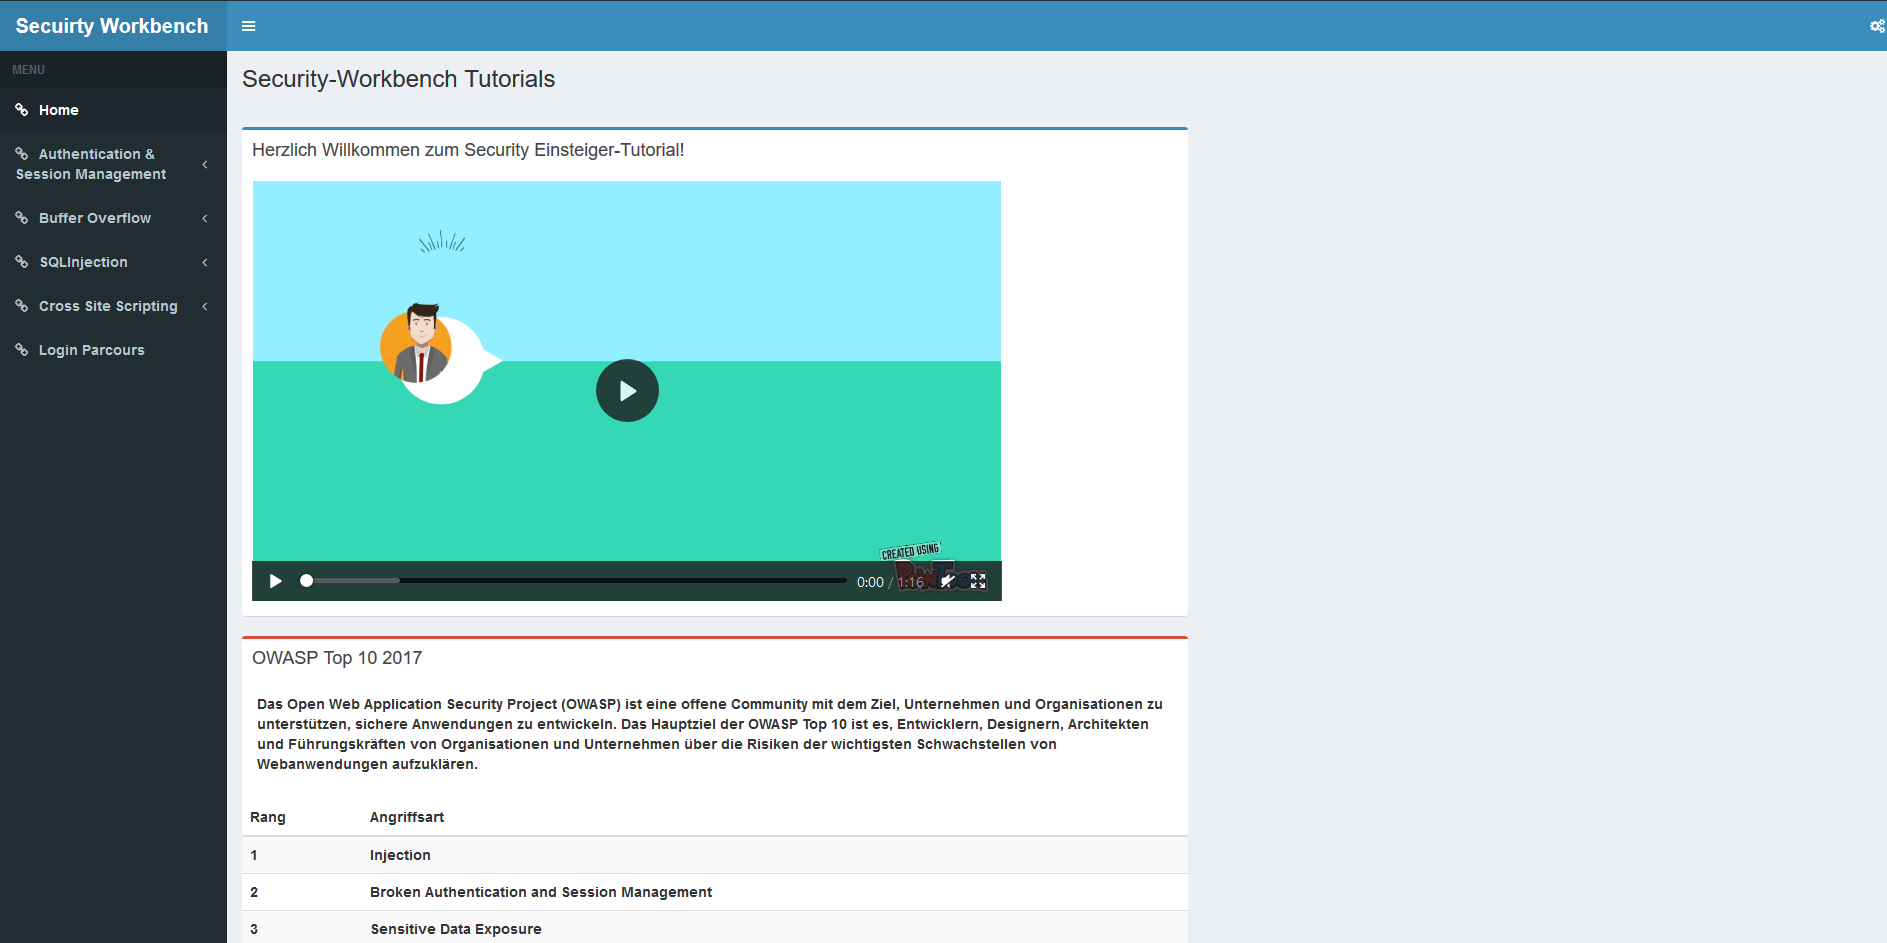
\includegraphics[width=\textwidth]{images/Installation/startseite.png}
	\caption{Nach erfolgreicher Installation, wird diese Startseite angezeigt}
	\label{fig:startseite}
\end{figure}

\section{Installationsanleitung mit Docker}
\label{sec:InstallWithDocker}

Die Installation der Web-Anwendung mithilfe des bereits konfigurierten Docker-Containers benötigt zuerst die Installation von Docker. Dies kann über den Package-Manager mit \colorbox{altgray}{\lstinline|apt-get install docker|} durchgeführt werden. Danach sollte, wie in Kapitel \ref{sec:Install} beschrieben, das GitHub-Repository geklont werden. Dort befindet sich der Ordner \colorbox{altgray}{\lstinline|PROJEKTROOT/Projekte/Docker/server |} der den Container mit allen benötigten Dienste bereitstellt. Dieses Verzeichnis muss nun auf den Desktop des Root-Users kopiert werden. Aus dem eben kopierten Ordner muss das StartUp.sh ebenfalls in das Desktop Verzeichnis verschoben werden. Dieses Skript wird dazu verwendet, den Docker-Container für die Web-Anwendung zu starten, bzw. wenn der Container noch nie gestartet wurde wird das Image des Containers erstellt. Zudem startet es alle benötigten Dienste. Es wird hier auch ein VSFTPD-Dienst gestartet. Dies ist ein FTP-Server, der nicht zwingend installiert werden muss, daher kann diese Zeile auskommentiert werden.\medskip

Nun müssen auch hier die Daten der Web-Applikation aus dem Verzeichnis \colorbox{altgray}{\lstinline|PROJEKTROOT/Projekte/SecWorkbench/html|} in den Ordner \colorbox{altgray}{\lstinline|/var/www/html|} kopiert werden. An dieser Stelle sollten die Berechtigungen mit dem Befehl \colorbox{altgray}{\lstinline|sudo chown -R www-data:www-data /var/www/html/|} aktualisiert werden. Danach kann man den Container starten, indem man das Skript StartUp.sh in der Kommandozeile aufruft. Hier sollte eine Ausgabe wie in Abbildung \ref{fig:startUp} angezeigt werden.

\begin{figure}[H]
	\centering
	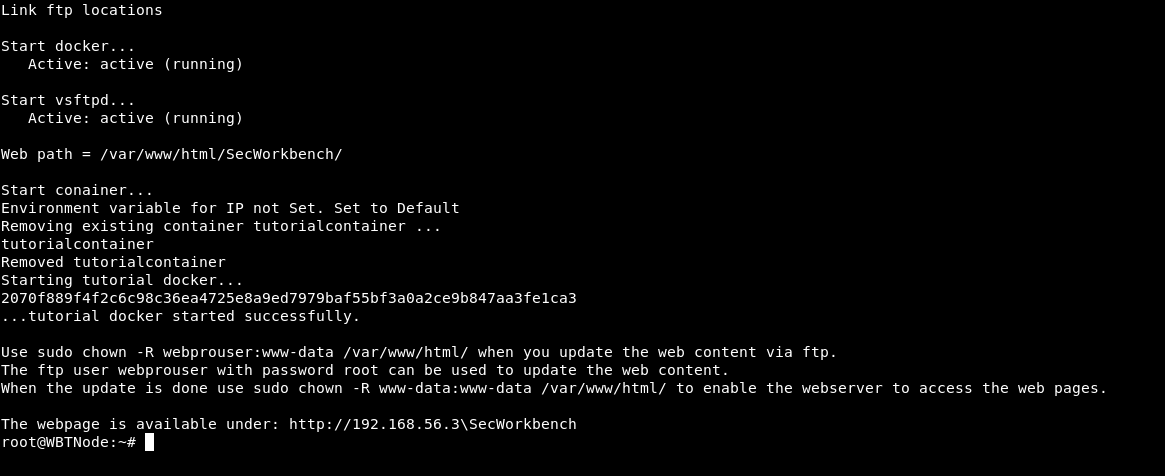
\includegraphics[width=\textwidth]{images/Installation/startUp.png}
	\caption{Die Ausgabe des Start-Skriptes nach erfolgreichem Start des Docker Containers}
	\label{fig:startUp}
\end{figure}

\section{Nutzung der virtuellen Maschine}

Die bereitgestellte virtuelle Maschine ist ein x64 Kali-Linux. Hier sind bereits alle Dienste vorinstalliert und konfiguriert. Des Weiteren wird der Root-User (ohne Passwort) automatisch beim Start der VM eingeloggt. Das Skript StartUp.sh wird beim Login des Root-Users aufgerufen, sodass die Website kurz nach dem Login erreichbar ist. Für die automatische Ausführung des Docker-Skripts dient die Konfigurationsdatei  \colorbox{altgray}{\lstinline|/etc/init/SecWorkbenchJob.conf|}. Die Ausgabe des Skriptes ist in einer maximierten Shell zu sehen, dabei wird auch die URL der Web-Applikation angezeigt. Dies ist in Abbildung \ref{fig:startUp} zu sehen.\medskip

In der VM wird die Web-Anwendung in einem Docker-Container betrieben. Dieser stellt den Apache-Webserver und die MySQL-Datenbank bereit. Dadurch wird beim Starten der virtuellen Maschine immer eine initiale Datenbasis für die Tutorials bereitgestellt. Um nachsehen zu können, ob der Container richtig gestartet wurde, ist es möglich alle gestarteten Container durch das Kommando \colorbox{altgray}{\lstinline|docker ps|} anzeigen zu lassen. Hier sollte ein Container mit dem Namen tutorialcontainer mit dem Status Up zu sehen sein.\newpage

Sollte es zu einem Fehler kommen bei dem der Container abstürzt, kann dieser mit den folgenden Befehlen wieder neu gestartet werden:

\begin{enumerate}
	\item \bashCommand{docker stop tutorialcontainer}
	\item \bashCommand{docker rm tutorialcontainer}
	\item \bashCommand{'/root/Desktop/server/tutorialDockerControl.sh' start}
\end{enumerate}

Der erste Befehl stellt sicher, dass der Container gestoppt wird. Danach soll der Container gelöscht und mit dem Start-Skript neu erstellt und gestartet werden. Sollten Modifikationen am Container nötig sein, muss vor dem Neustart noch der Befehl \bashCommand{docker rmi tutorialimage} durchgeführt werden. Dieser löscht das Image, sodass aufbauend auf dem grundlegenden Debian-Images die Änderungen mit übernommen werden.\medskip

Sollten sich die Quell-Dateien ändern, so können diese über das Git-Repository aktualisiert werden. Dazu wechselt man in das Verzeichnis\\ \bashCommand{/root/INF-M-Projekt-Security-Workbench/} und führt zunächst den Befehl \bashCommand{git pull} aus. Dadurch wird das lokale Repository auf den aktuellen Stand des GitHub-Repositorys gebracht. Als nächstes kopiert man den Inhalt des Pfads \\ \bashCommand{PROJEKTROOT/Projekte/SecWorkbench/html} nach \bashCommand{/var/www/html}. Danach muss der Container gestoppt und neu gestartet werden, siehe dazu die oben stehenden Befehle 1 und 3.\medskip

In der ausgelieferten VM, kann zudem das Repository per FTP aktualisiert werden. Im startUp.sh wurden die Kommentare entfernt, die den Start des FTP-Dienstes beim Boot der VM automatisch ausführen. Dabei wird in der startUp.sh der vsftpd Dienst gestartet, indem das Kommando \bashCommand{sudo service vsftpd start} ausführt wird. Für diesen Dienst ist der User webprouser bereits eingerichtet und besitzt das Passwort root. Um Schreibrechte außerhalb des Home-Verzeichnisses des Users zu bekommen muss hier der Unterordner \bashCommand{/home/webprouser/html/SecWorkbench/} auf \bashCommand{/var/www/html/SecWorkbench/} zeigen. Dies kann mit dem Befehl\\ \bashCommand{mount --bind /home/webprouser/html/SecWorkbench/ /var/www/html/SecWorkbench/} vorgenommen werden. Um nun per FTP-Daten schreiben zu können, muss man die Berechtigungen auf dieses Verzeichnis aktualisieren. Dazu führt man das Kommando \bashCommand{sudo chown -R webprouser /home/webprouser/html/} aus. Nun können per FTP-Client Quell-Dateien direkt in das Verzeichnis, dass die HTML-Ressourcen bereitstellt eingefügt werden. Ist der Upload fertig, muss man die Rechte des html-Verzeichnisses wieder an den Apache-User geben. Dies erreicht man mit dem Befehl \bashCommand{sudo chown -R www-data:www-data /var/www/html/}.
%!TEX root = ../document.tex
\chapter{Verwendete Tools}
Es folgt eine kurze Übersicht der Tools, die in den Beispielen mehrfach eingesetzt werden. Hier wird jeweils der Zweck des Tools und die Bedienung kurz demonstriert.

\section{Tool 1}

%!TEX root = ../document.tex
\chapter{Broken Authentication and Session Management}
\label{BrokenAuthenticationAndSessionManagement}

\section{Erklärung}
Diese Sicherheitslücke befindet sich im OWASP Top 10 Risk Rating 2017 auf dem 2. Platz (OWASP A2). 
Auf vielen Web-Applikationen wird eine Benutzerauthentifizierung mit Benutzername und Passwort benötigt, um deren Dienste zu nutzen. Beispiele hierfür sind Online-Shops, Social-Media-Plattformen und Online-Banking. 
\\
Für die Interaktion zwischen dem angemeldeten Benutzer und der Web-Applikation ist das Session-Management nötig, wobei die gesammelten Session-Informationen in Cookies unter der eindeutigen Session-ID der Benutzer-Session abgespeichert werden. Cookies werden vom Browser verwendet, um client-seitig Informationen abzuspeichern.
\\
Der technische Hintergrund ist die Zustandslosigkeit des HTTP-Protokolls. Das HTTP-Protokoll wird für die Kommunikation zwischen dem Client und dem Web-Server eingesetzt. Die Zustandslosigkeit führt dazu, dass der Web-Server Seitenaufrufe unabhängig voneinander interpretiert und keinen Zusammenhang herstellen kann. Mit Hilfe des Session-Managements werden die Seitenaufrufe eines Benutzers in einer Session einander zugeordnet. Die Session-ID ist eine lange und zufällige Zeichenkette, wobei sichergestellt werden muss, dass dieser Identifier eindeutig und nicht leicht zu erraten ist.
\\
Als mögliche Konsequenz von Fehlern in der Authentifizierung und dem Session-Management folgt die Kompromittierung oder Übernahme von Benutzerkonten.

\subsection{Fehler in der Authentifizierung}
Wenn die Passwort-Policy für die Registrierung nicht ausreichend streng ist, verleitet dies Benutzer dazu schwache Passwörter zu verwenden. Dadurch wird ein Brute-Force-Angriff möglich, wobei durch systematisches Probieren aller möglichen Kombinationen die Benutzernamen und dazugehörigen Passwörter fremder Benutzer erraten werden können.\\\\
Eine weitere Fehlerquelle ist die Verschlüsselung von Benutzername und Passwort. Wenn diese Daten im Klartext über das HTTP-Protokoll versendet werden, ist es einem Angreifer möglich die Kommunikation abzuhören. Wenn beim Abspeichern der Benutzerdaten auf Hash-Verfahren bzw. Verschlüsselung verzichtet wird, sind diese Daten ungeschützt vor anderen Sicherheitslücken wie beispielsweise SQL-Injections.\\
Teilweise gibt der Web-Server aussagekräftige Informationen über bereits bestehende Benutzerkonten Preis, sodass ein fremdes Benutzerkonto übernommen werden kann. Bei der Konto-Erstellung oder "Passwort-Zurücksetzen"-Funktion kann ggf. ein bestehender Benutzername ermittelt werden. Der Benutzername stellt bereits die erste Hälfte der Lösung des Benutzername-Passwort-Rätsels dar.

\subsection{Fehler im Session-Management}
Ist die Wahl der Session-ID nicht ausreichend zufällig gestaltet, besteht die Möglichkeit, dass eine gültige Session-ID erraten wird. Wenn zudem die Session-ID als Parameter in der URL übergeben wird, ist es einem Dritten möglich die Session zu übernehmen. Dieser Dritte kann dadurch alle Funktionen der Web-Applikation mit den Berechtigungen des angemeldeten Benutzers verwenden. Wird die URL unverschlüsselt übertragen, kann ein Angreifer ebenfalls eine fremde Session-ID ermitteln und die Session eines angemeldeten Benutzers übernehmen. Das HTTPS-Protokoll bietet eine Verschlüsselung für diese Problematik.\\
Wenn Session-IDs nach dem Abmelden eines Benutzers nicht auf ungültig gesetzt werden, können diese zur Wiederherstellung der Anwender-Session missbraucht werden. Ebenso werden Session-IDs zu vorhersehbar, wenn diese sich nicht mit erneuter Anmeldung ändern.\\
Wenn das HttpOnly-Attribut nicht gesetzt wird, ist das Auslesen des Session-Cookies über Skriptsprachen möglich. Im Rahmen eines XSS-Angriffs kann die Session-ID eines anderen Benutzers ermittelt werden. 

\subsection{Gegenmaßnahmen}
Die Authentifizierungsfunktion ist so zu gestalten, dass nach wiederholter Fehleingabe der Anmeldedaten das Benutzerkonto oder die Aufrufer-IP temporär gesperrt werden.\\
Außerdem sollte weder bei der Registrierung noch bei der "Passwort-Vergessen"-Funktion eine aussagekräftige Rückmeldung über bereits existierende Benutzernamen gegeben werden. Wenn dies aus Gründen der Benutzerfreundlichkeit nicht möglich ist, sind zumindest automatisierte Abfragen zu unterbinden.\\\\
Die Übermittlung der Anmeldedaten sollte ausschließlich verschlüsselt mit TLS und die Speicherung der Passwörter in gehashter Form mit geeigneten kryptographischen Funktionen gestaltet werden.\\
Session-IDs sind ausreichend zufällig zu wählen, nicht unverschlüsselt zu übertragen und bei einer Abmeldung serverseitig zu beenden. Zum Erzwingen der Verschlüsselten Übertragung der Session-ID wird das Secure-Attribut des Session-Cookies aktiviert. Außerdem ist es ratsam das HttpOnly-Attribut zu setzen, um ein Auslesen des Cookies mittels JavaScript zu verhindern.\\
Um Session-Übernahmen zu vermeiden, ist es darüber hinaus möglich, die Session des Anwenders mit spezifischen Nutzermerkmalen, beispielsweise dem entsprechenden User-Agent oder der IP-Adresse zu verknüpfen.\\
Neben diesen Standardmaßnahmen sind auch die von der OWASP formulierten Anforderungen an Authentifizierung und Session-Management umzusetzen. Diese sind in den OWASP Application Security Verification Standards beschrieben.\\
\\
Quelle:\\ https://www.datenschutz-notizen.de/owasp-top-ten-a2-fehler-in-authentifizierung-und-session-management-2713238/

\section{Übungen}
\subsection{Registrierung}
Das Lernziel der ersten Übung zum Thema Registrierung ist es, dem Anwender gängige Passwortregeln aufzuzeigen. Inhalt der Übung ist es, sich erfolgreich zu registrieren unter Einhaltung gängiger Passwortregeln. Die Startseite der Übung ist Abbildung \ref{fig:Aufgabe 1 Registrierung} zu entnehmen.\\


\begin{figure}[]
	
	\centering
	
	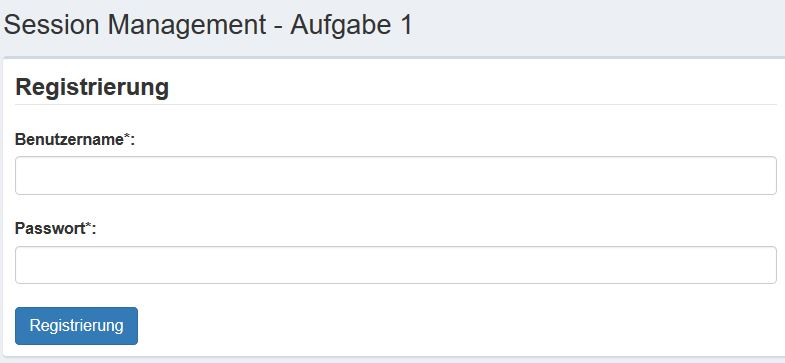
\includegraphics[width=1.0\linewidth]{images/BrokenAuthenticationAndSessionManagement/Registrierung_Start}
	
	\caption[Aufgabe 1: Registrierung nach gängigen Passwortregeln.]{Registrierung nach gängigen Passwortregeln.}
	
	\label{fig:Aufgabe 1 Registrierung}
	
\end{figure}
\noindent In dieser Übung werden zwei Hinweise zur Verfügung gestellt. Der erste Hinweis ist, dass das gewählte Passwort den allgemein üblichen Regeln zu entsprechen hat, damit die Registrierung erfolgreich durchgeführt werden kann. Im zweiten Hinweis werden die verwendeten Passwortregeln aufgelistet: Länge von mind. 8 Zeichen, mind. ein Großbuchstabe, mind. ein Kleinbuchstabe und eine Zahl. \\
Nach erfolgreicher Registrierung wird der Benutzer auf die in Abbildung \ref{fig:Aufgabe 1 Abschluss} dargestellte Seite weitergeleitet und hat die Aufgabe erfolgreich gelöst.\\
\begin{figure}[H]
	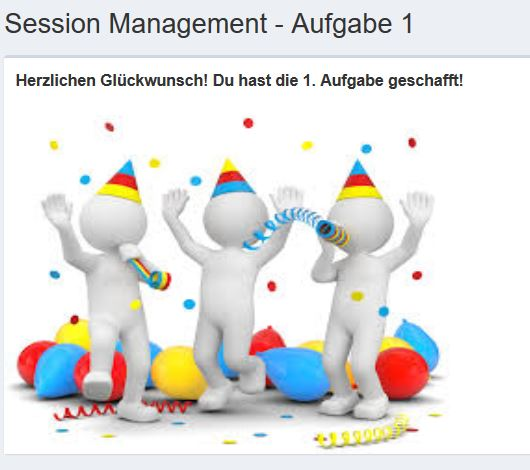
\includegraphics[width=1.0\linewidth]{images/BrokenAuthenticationAndSessionManagement/Registrierung_Ende}
	\caption[Landing-Page nach erfolgreicher Registrierung.]{Landing-Page nach erfolgreicher Registrierung.}
	\label{fig:Aufgabe 1 Abschluss}
\end{figure}
\subsection{Login}
Das Ziel der zweiten Übung liegt darin aufzuzeigen, wie leicht Passwörter zu erraten sind, wenn die gängigen Passwortregeln nicht einzuhalten sind. Es gibt sehr beliebte und einfache Benutzername- und Passwort-Kombinationen, die in dieser Übung ausgenutzt werden.\\ 
Die Aufgabenstellung ist deshalb so gewählt, dass sich der Benutzer mit einem fremden, unbekannten Benutzerkonto anmelden soll. Dabei sind Benutzername und Passwort zu erraten. \\
\begin{figure}[H]
	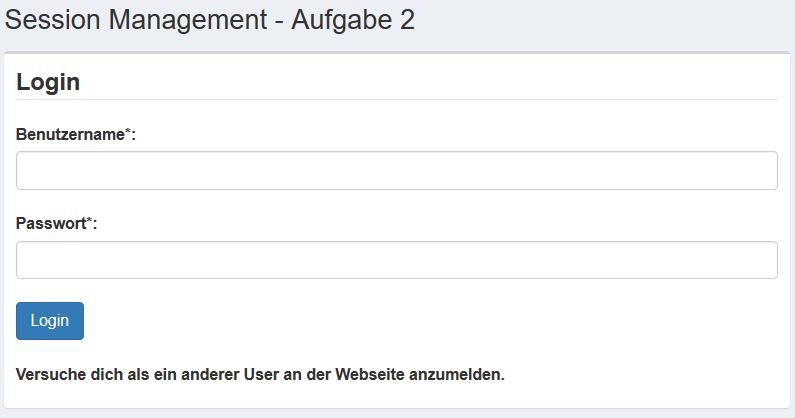
\includegraphics[width=1.0\linewidth]{images/BrokenAuthenticationAndSessionManagement/Login_Start}
	\caption[Aufgabe 2: Login.]{Aufgabe 2: Login.}
	\label{fig:Aufgabe 2 Login}
\end{figure}
\noindent Bei Bedarf werden zwei Hinweise gegeben. Der erste Hinweis ist, dass es sich hier um sehr einfache, beliebte Benutzernamen und Passwörter handelt. Wenn dieser Tipp nicht ausreicht, wird im zweiten Hinweis ein existierendes Passwort ('admin') vorgegeben. Zu diesem Benutzername würde das Passwort 'admin' passen. Es gibt jedoch auch andere Kombinationen: z.B. Benutzername 'benutzer' und als Passwort 'passwort1' oder 'fußballfan' und 'schalke04'.\\
Einige dieser beliebten Benutzernamen und Passwörter sind in der Datenbank der Webseite hinterlegt.\\\\\\\\\\\\
Bei erfolgreicher Anmeldung mit einem fremden Benutzerkonto, gelangt der Benutzer zur letzten Seite dieser Übung:
\begin{figure}[H]
	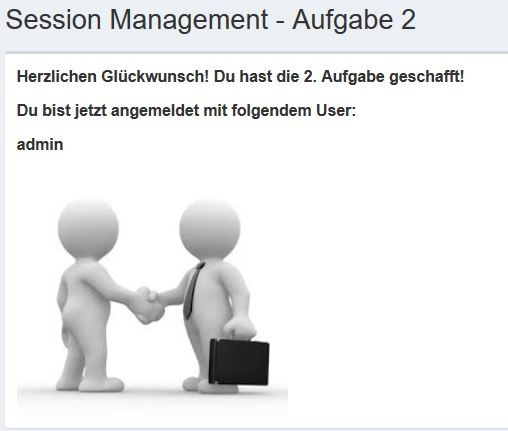
\includegraphics[width=1.0\linewidth]{images/BrokenAuthenticationAndSessionManagement/Login_Ende}
	\caption[Landing-Page nach erfolgreichem Login.]{Landing-Page nach erfolgreichem Login.}
	\label{fig:Aufgabe 2 Abschluss}
\end{figure} 
\noindent Durch das Erraten von Benutzername und Passwort, ist es möglich die Funktionen der Webapplikation mit den Berechtigungen des fremden Benutzerkontos zu nutzen. In unserer Übung wird das jedoch nicht mehr abgefragt.
\subsection{Logout}
Das Lernziel der dritten Übung ist die Erkenntnis, dass nach einem Logout die Session zwingend beendet werden muss und die dazugehörigen Daten nicht mehr verfügbar sein dürfen.\\\\\\
Die Aufgabenstellung liegt darin, nach dem Logout ohne erneute Anmeldung zurück zu der Webseite als angemeldeter Benutzer zu gelangen.\\ 
\begin{figure}[H]
	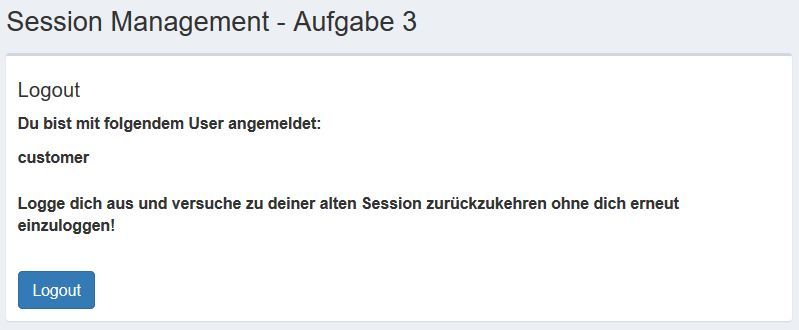
\includegraphics[width=1.0\linewidth]{images/BrokenAuthenticationAndSessionManagement/Logout_Start}
	\caption[Aufgabe 3: Logout.]{Aufgabe 3: Logout.}
	\label{fig:Aufgabe 3 Logout}
\end{figure}



\noindent Durch das Klicken auf den Logout-Button erfolgt eine Weiterleitung zur Logout-Seite. Diese ist in Abbildung \ref{fig:Aufgabe 3 Abschluss} abgebildet.\\\\
\begin{figure}
	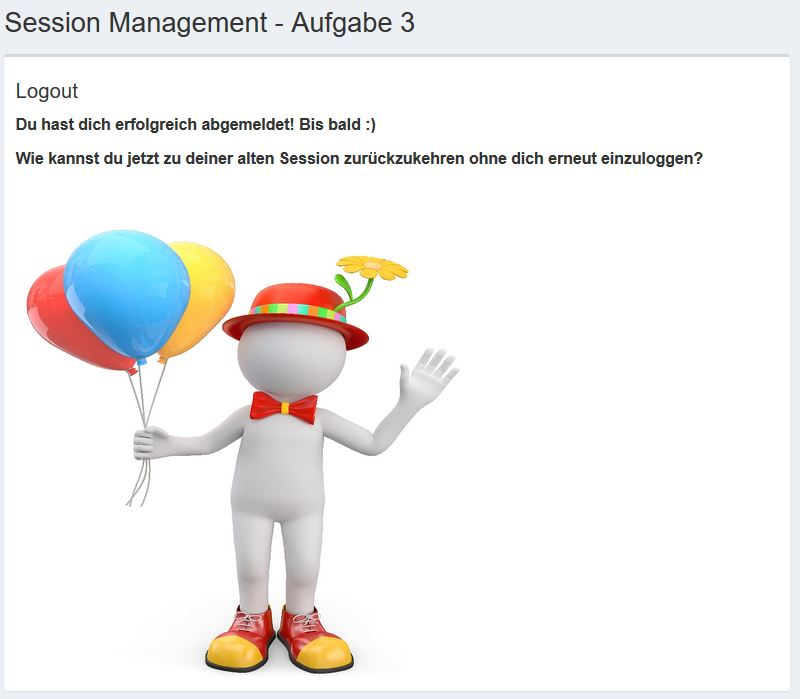
\includegraphics[width=1.0\linewidth]{images/BrokenAuthenticationAndSessionManagement/Logout_Mitte}
	\caption[Logout-Seite.]{Logout-Seite.}
	\label{fig:Aufgabe 3 Abschluss}
\end{figure}

\noindent Hier wird der Hinweis, dass der Browser eine 'zurück'-Funktion bietet, bei Bedarf zur Verfügung gestellt.\\
Wird die Funktion des Browsers ausgenutzt, gelangt der Benutzer wieder zur Startseite der Übung und erscheint als angemeldeter Benutzer. Somit ist die Übung erfolgreich absolviert.\\\\\\\\\\\\\\\\\\\\\\\\\\
\subsection{URL-Manipulation}
Mithilfe der letzten Übung wird gezeigt, dass Session-Attribute und die Session-ID nicht sichtbar übertragen werden sollten, wie z.B. in der URL. Zudem darf die Session-ID nicht spechend wie beispielsweise der Benutzername gewählt werden. Es ist besser, wenn die Session-ID einer willkürlichen Zeichenfolge entspricht.\\
Die Aufgabenstellung besteht darin, das Benutzerkonto des Admins zu übernehmen. Aktuell ist der Benutzer 'customer' angemeldet.\\
\begin{figure}[H]
	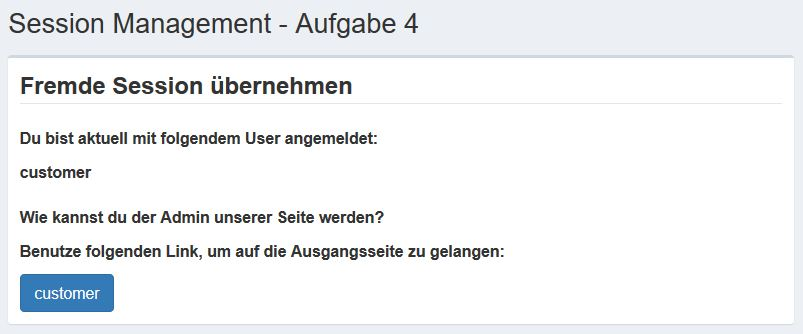
\includegraphics[width=1.0\linewidth]{images/BrokenAuthenticationAndSessionManagement/URL_Start}
	\caption[Aufgabe 4: URL-Manipulation.]{Aufgabe 4: URL-Manipulation.}
	\label{fig:Aufgabe 4 URL-Manipulation}
\end{figure}
\noindent Durch Betätigung des Buttons 'customer', gelangt der Benutzer zur Ausgangsseite:
\begin{figure}[H]
	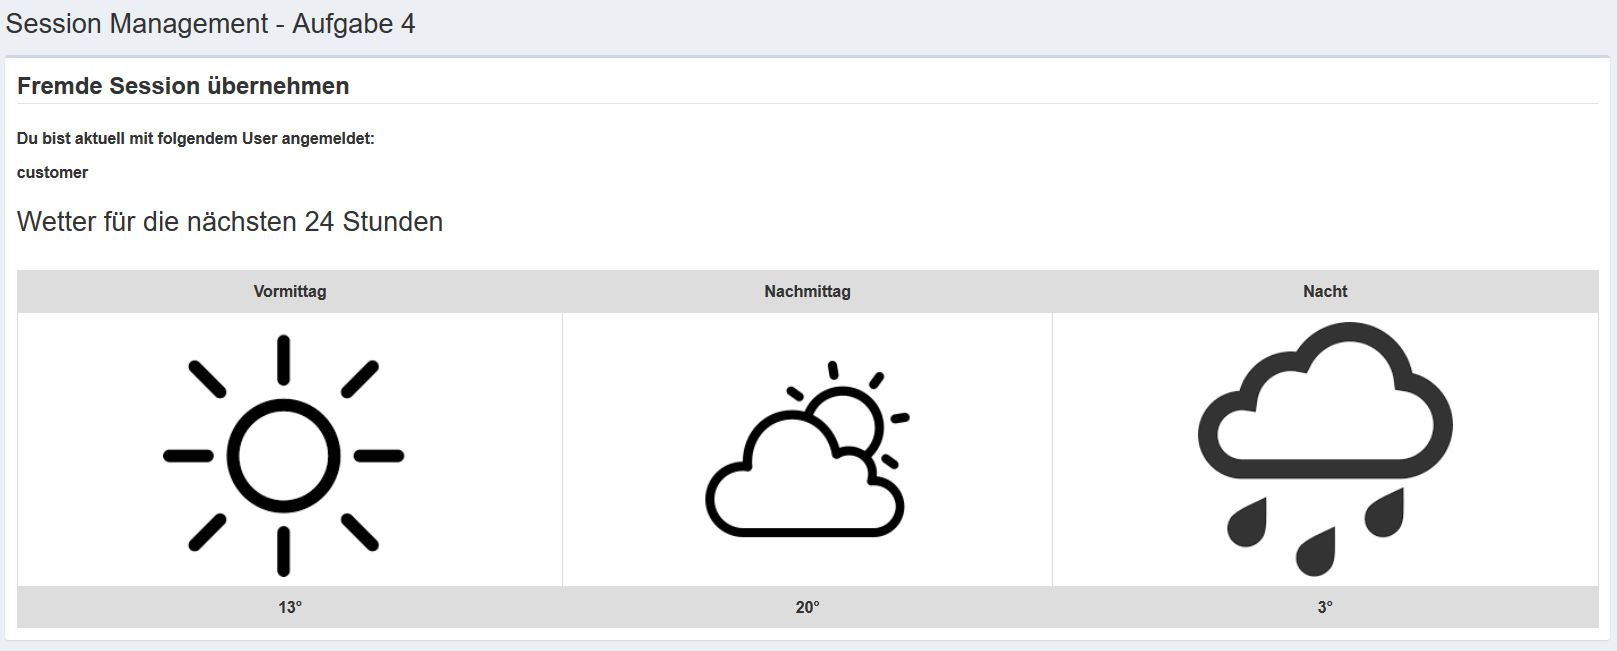
\includegraphics[width=0.95\linewidth]{images/BrokenAuthenticationAndSessionManagement/URL_customer}
	\caption[Aufgabe 4: Ausgangsseite des Customers.]{Aufgabe 4: Ausgangsseite des Customers.}
	\label{fig:Aufgabe 4 Ausgangsseite des Customers}
\end{figure}
\noindent Auf der Ausgangsseite werden zwei Hinweise angeboten. Der erste Tipp, weißt auf die Unterschiede des GET- und POST-Requests des HTTP-Protokolls hin. Der zweite Tipp lenkt die Aufmerksamkeit des Anwenders auf die Parameter der URL, die zu manipulieren sind.\\
Die Parameter in der URL entsprechen dem Lösungsweg, da hier der Username hinterlegt ist.
\begin{figure}[H]
	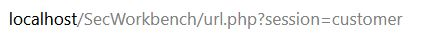
\includegraphics[width=1.0\linewidth]{images/BrokenAuthenticationAndSessionManagement/URL_customer_url}
	\caption[Aufgabe 4: URL der Ausgangsseite des Customers.]{Aufgabe 4: URL der Ausgangsseite des Customers.}
	\label{fig:Aufgabe 4 URL der Ausgangsseite des Customers}
\end{figure} 
\noindent Wird der Wert des Session-Parameters von 'customer' auf 'admin' geändert, gelang der Benutzer zur Session des Admins.
\begin{figure}[H]
	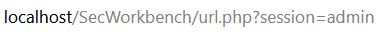
\includegraphics[width=1.0\linewidth]{images/BrokenAuthenticationAndSessionManagement/URL_admin_url}
	\caption[Aufgabe 4: URL der Ausgangsseite des Admins.]{Aufgabe 4: URL der Ausgangsseite des Admins.}
	\label{fig:Aufgabe 4 URL der Ausgangsseite des Admins}
\end{figure}
\noindent Für den Admin ist der Wetterbericht der nächsten drei Tage sichtbar, der Kunde sieht jedoch nur das Wetter der nächsten 24 Stunden. Wenn der Benutzer auf dieser Seite angelangt ist, hat er die letzte Übung erfolgreich abgeschlossen.
\begin{figure}[H]
	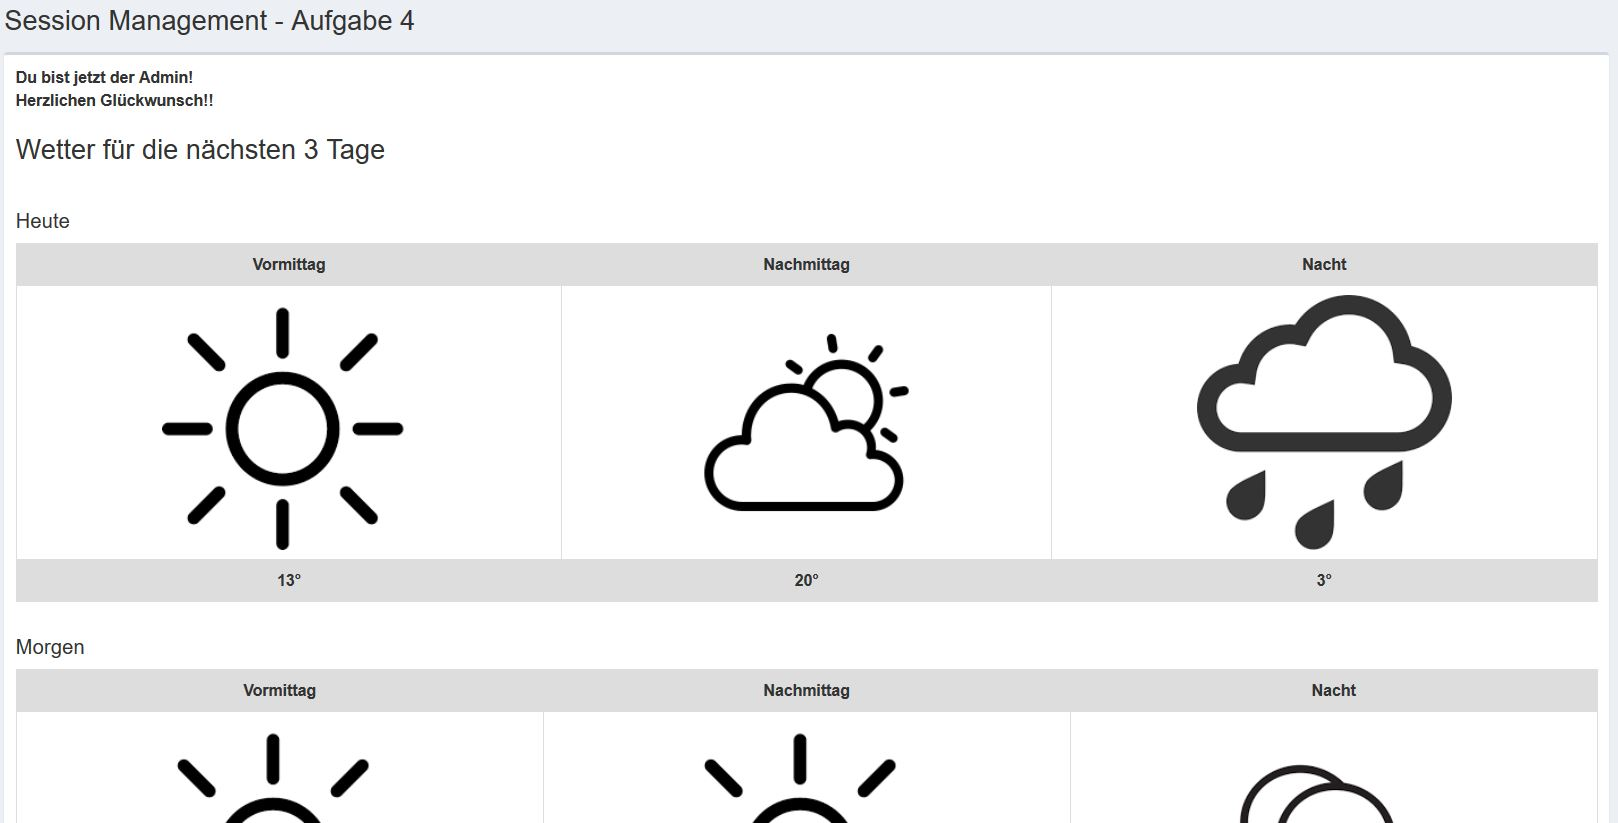
\includegraphics[width=1.0\linewidth]{images/BrokenAuthenticationAndSessionManagement/URL_admin}
	\caption[Aufgabe 4: Ausgangsseite des Admin.]{Aufgabe 4: Ausgangsseite des Admin.}
	\label{fig:Aufgabe 4 Ausgangsseite des Admin}
\end{figure}
%!TEX root = ../document.tex
\chapter{Buffer Overflow}
\subsubsection*{Von: Marwin Sedlmayer, Marco Egener(Unterkapitel PHP-Shell)}
Ein Buffer Overflow ist ein Angriff, bei dem einem Puffer zu viele Werte übergeben werden. Dadurch ist es möglich die Werte anderer Variablen oder Adressen zu überschreiben. \\
Im folgenden Kapitel wird die Portierung und Weiterentwicklung der Buffer Overflow Beispiele aus dem Wintersemester 16/17 auf die Broken Web Application des diesjährigen Semesters beschrieben.

Hierbei wurden die Beispielangriffe um Erklärungen und Anleitungen erweitert, sowie eine Übersichtsseite eingefügt. Auch die angreifbaren Files wurden leicht verändert, so dass auch ohne einen Debugger verständlich ist, wie diese Angriffsart funktioniert.
\section{Übersichtsseite}
Auf der Übersichtsseite wird die generelle Funktion eines Buffer Overflow Angriffs erklärt. Des Weiteren wird ein sehr berühmter Angriff, der Heartbleed - Angriff, in einem Comic mit Erklärung erläutert. Die Übersichtsseite ist in folgender Grafik dargestellt.

\begin{figure}[H]
	\centering
	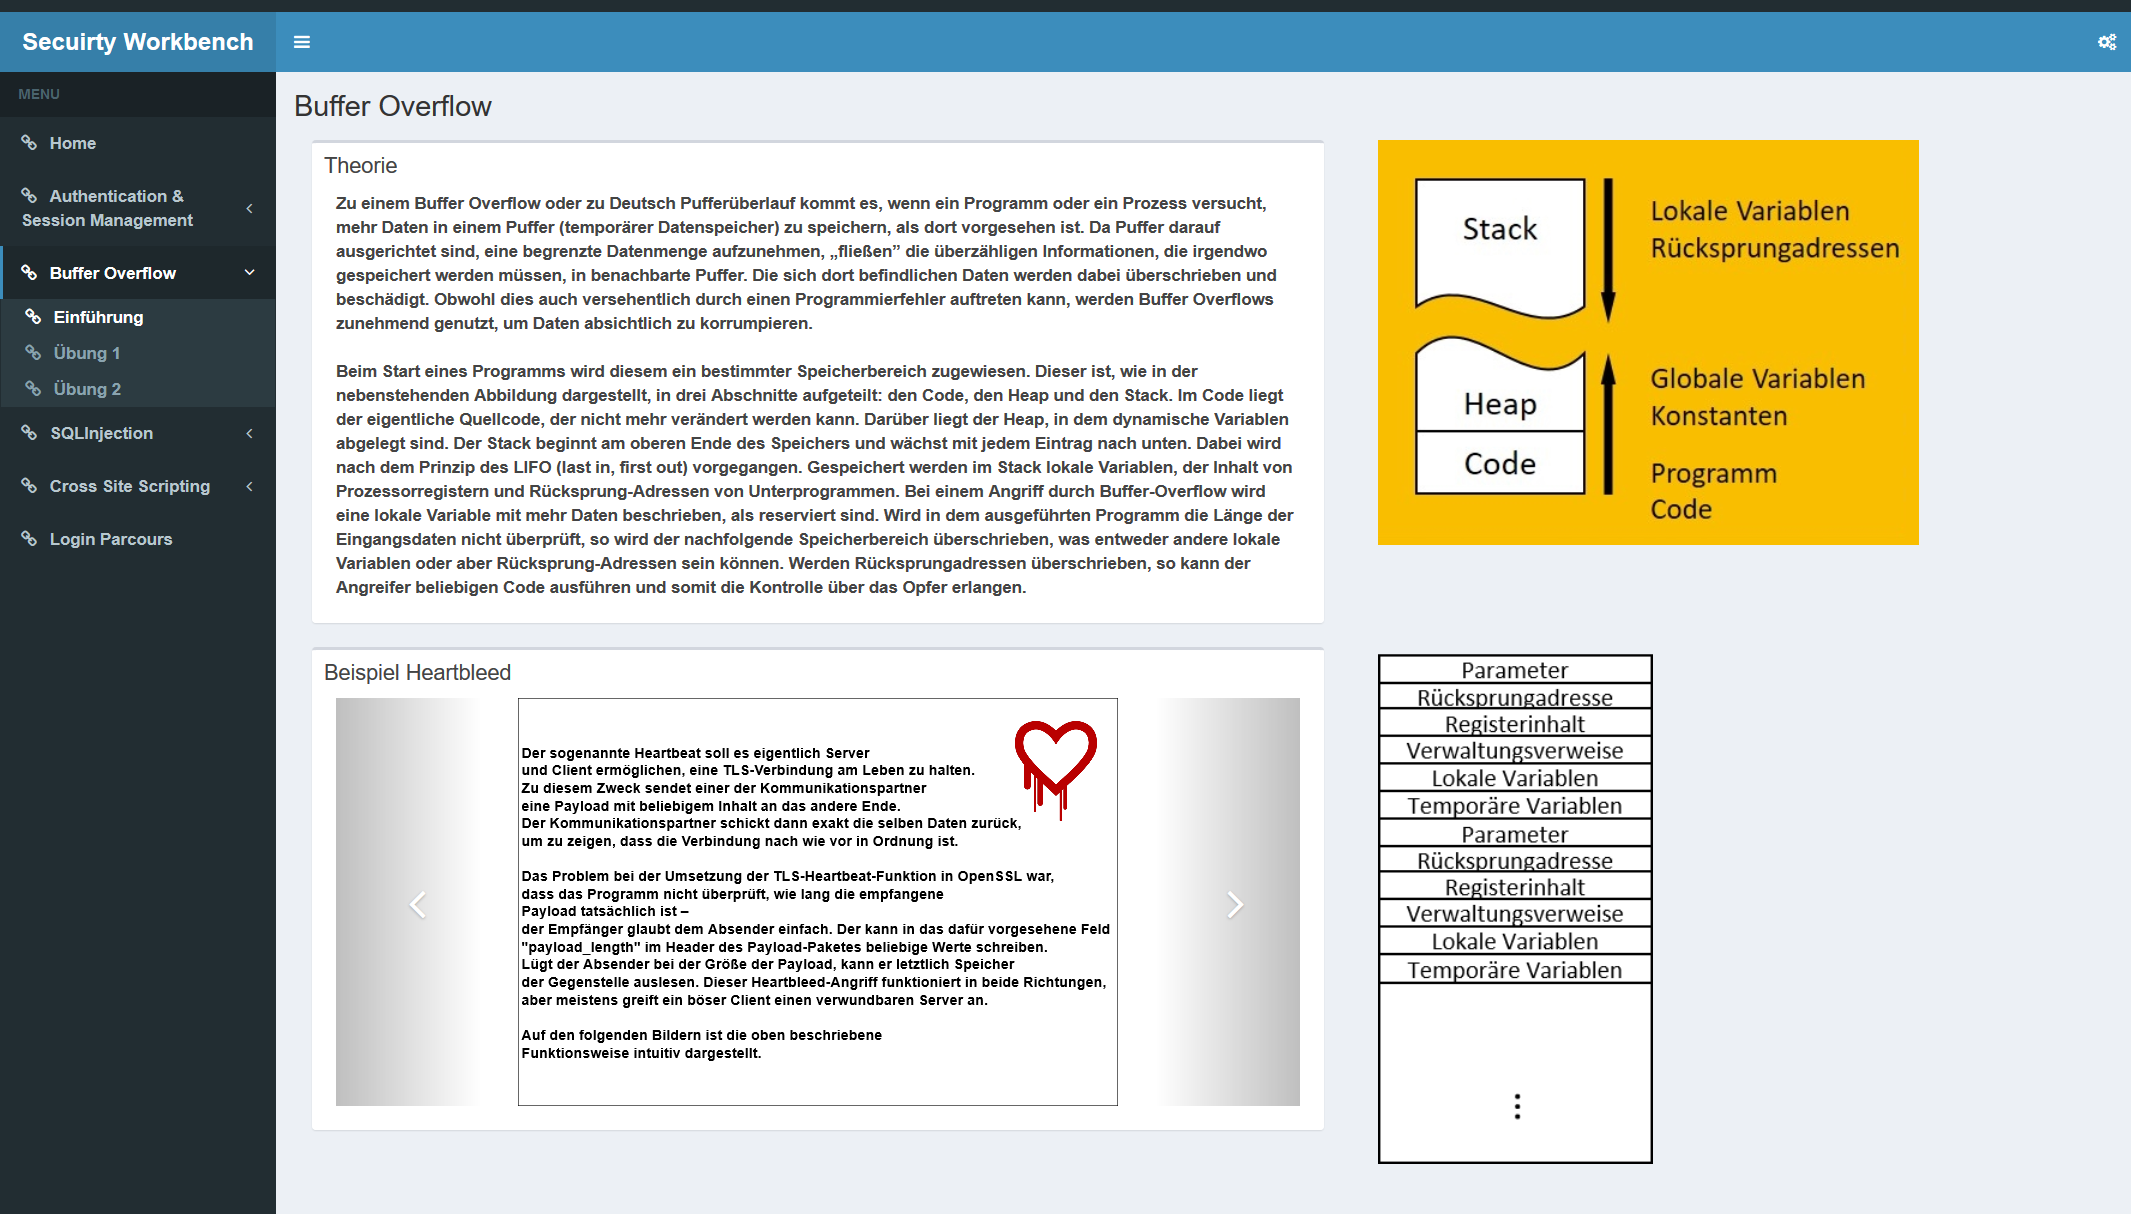
\includegraphics[width=\textwidth]{images/Bufferoverflow/Uebersichtsseite.PNG}
	\caption{Die Übersichtsseite der Buffer Overflow Übungen}
	\label{fig:BO_Overview}
\end{figure}

\section{Übung 1}
\subsection{C-File}
Die erste Übung ist ein sehr einfacher Buffer Overflow. Ein Eingabeparameter wird mit einem zufällig generierten Passwort verglichen und sollten sie identisch sein, wird ein Authentifizierungsflag gesetzt und man hat sich \glqq{}authentifiziert\grqq{}. Dies wird durch eine Erfolgsmeldung und das Ausgeben der Eingabeparameter und Variablen simuliert. Ziel der Übung ist es sich ohne Kenntnis des Passworts zu authentifizieren.
Der Code wird in folgendem Listing dargestellt.

\lstset{language=C, caption={Erstes Buffer Overflow Beispiel}, label=lst:BO_FE}
\begin{lstlisting}
int main(int argc, char *argv[80])
{
    //flag for authentication check
    int authflag = 0;
    //buffer for solution word
    char solution[21];
    //buffer for user input
    char buffer[8];

    //write user input to buffer
    strcpy(buffer, argv[1]);

    char randstr[8];
    srand ( time(NULL) );

    //create random Password
    sprintf(randstr, "%d", rand() );

    //check if input = Password
    if(strcmp(randstr,buffer)== 0)
    {
        printf("Really...?\n");
        //yeah we got the right pw so we are now authenticated
        authflag = 1;
    }

    //check for Authentication
    if(authflag != 0)
    {
        printf("Das Passwort ist: %s\n", randstr);

        printf("Der Eingabepuffer ist: %s\n", buffer);

        printf("Das Authflag hat den Wert: %d\n", authflag);

        printf("Das Lösungswort ist : %s\n", solution);
    }
    else
    {
        printf("Fehler: Login fehlgeschlagen!");
    }
}
\end{lstlisting}
Im Vergleich zu letztem Semester wurde das C-File ein wenig verändert, die Änderungen sind im Folgenden aufgelistet.
\begin{itemize}
	\item \textbf{Seed der Funktion rand()} In der Programmiersprache C ist es nur sehr schwer möglich Zufallszahlen zu generieren. Die gebräuchlichste Methode ist dabei die Funktion rand(), die allerdings auch keine echten Zufallszahlen erzeugt, für dieses Beispiel jedoch ausreichend ist. Wichtig bei der Benutzung dieser Funktion ist indes, dass sie einem sogenannten Seed, der vor Aufruf der Funktion rand() gesetzt werden muss, einen \glqq{}zufälligen\grqq{} Wert zuweist. Das bedeutet, dass die Funktion für den gleichen Seed immer den gleichen Rückgabewert lieft. \\
	Hier hatte das Team des letzten Semesters vergessen den Seed bei jedem Aufruf des Programms zu verändern. In der jetzigen Version wurde deshalb in der Zeile 14 des Programms ein Seed mit der aktuellen Systemzeit gesetzt.
	\item \textbf{Ersetzen des alten Lösungsworts} War der Angriff erfolgreich, so wurde in der alten Version ein Lösungswort ausgegeben. Der Speicherplatz dafür war allerdings mithilfe der Funktion malloc() dynamisch alloziert und damit liegt das Lösungswort auf dem Heap und nicht auf dem Stack, der in diesem Beispiel angegriffen wird. DAs Lösungswort war also nicht überschreibbar und hatte in seinem initialzustand leider keine Bedeutung. \\
	Dieses Lösungswort wurde durch eine Aussagekräftige Ausgabe ersetzt (siehe Zeilen 30ff).
	\item \textbf{Einfügen einer Fehlermedlung} Im alten Programm gab es keine Rückmeldung, sollte der Angriff gescheitert sein. Wird das Programm lokal in einem Debugger ausgeführt, ist das auch kein Problem, da hier eindeutig ersichtlich ist, dass das Programm läuft. Für die Ausführung mithilfe einer Client / Server Architektur, wo in erster Instanz kein Debugger zur Verfügung stand, ist eine Fehlermeldung als Bestätigung des Fehlschlags sehr hilfreich. Diese wurde in der Zeile 40 eingefügt.
\end{itemize}

Um den Angriff erfolgreich durchzuführen, ist es lediglich nötig als Eingabeparameter einen mindestens 30 Zeichen langen String zu übergeben. Dies ist natürlich ein sehr einfaches Beispiel, allerdings spiegelt es sehr gut wider, welche gravierenden Auswirkungen ein einfacher Programmierfehler haben kann.

\subsection{Website}
Auf der Übungsseite befindet sich eine kurze Erklärung des Beispiels, sowie der Code des Programms, der mithilfe von prism direkt aus dem C-File ausgelesen wird. Über die weiter unten befindliche Eingabemaske kann der Angriff ausgeführt werden. Die Ausgabe des Programms wird in der nebenstehenden Box angezeigt. Das Programm wird mit php auf dem Server ausgeführt, der String des Eingabefelds wird per Formular zur Verfügung gestellt.

Sollte das Beispiel für die Studierenden nicht lösbar sein, ist eine dreistufige Tippstruktur vorgesehen, in der den Studierenden je nach Level abstrakte Hinweise gegeben werden, bzw. die Lösung verraten wird.

\subsection{PHP-Shell}
Die integrierte PHP-Shell, soll dem Anwender eine Möglichkeit bieten, den Programmablauf und die Speicherstruktur mit verfolgen zu können. Die PHP-Shell lässt sich wie ein Linux Terminal bedienen. Dazu kann im Eingabefeld das Bash-Kommando eingegeben und mit einem Klick auf den Button \glqq execute command\grqq\, auf dem Server ausgeführt werden. Hierbei werden die Daten mittels POST an den Server geschickt. Der Server startet dabei ein Terminal mit dem entsprechenden Kommando und schließt diesen Prozess nach der Abarbeitung der Befehle. Dabei ist zu beachten, dass das Terminal unter Root-Rechten ausgeführt wird.\medskip

Für dieses Beispiel ist der Gnu Debugger (GDB) hilfreich, um die Speicheradressen der zu überschreibenden Variablen heraus zu finden. Damit kann die Größe der Variablen und somit auch die Länge der Eingabe ermittelt werden. Dies kann z. B. durch folgendes Kommando angezeigt werden:

\bashCommand{gdb -q -batch -ex \glqq break 15\grqq\, -ex \glqq run\grqq\, -ex \glqq p \&authflag\grqq\, -ex \glqq p \&buffer\grqq}\\ \bashCommand{./App\_Data/FirstExample}\medskip

Die oben stehende Anweisung veranlasst, dass in Zeile 15 des Codes ein Breakpoint gesetzt wird. Dabei werden keine Aufrufparameter übergeben, es wird lediglich die Adressen der Variablen authflag und buffer ausgegeben. Hier gilt es zu beachten, dass die Shell nach jedem Ausführen von Kommandos wieder geschlossen wird. Daher muss der GDB im Batch-Modus bedient werden. 

\section{Übung 2}
\subsection{C-File}
Die zweite Übung ist im Vergleich zur ersten ein wenig schwieriger gestaltet. Die Länge des Eingabepuffers wird zwar immer noch nicht überprüft, aber als erste Maßnahme gegen einen Angriff wurde eine Magic Number als Prüfinstanz eingefügt. Diese wurde so platziert, dass sie bei einem Buffer Overflow vor dem Authentifizierungsflag liegt. Damit muss ein Angriff auch diese Magic Number überschreiben. Die restliche Funktion des Programms ist identisch zum ersten Beispiel. \\
Der Code des zweiten Beispiels wird in folgendem Listing dargestellt.

\lstset{language=C, caption={Zweites Buffer Overflow Beispiel}, label=lst:BO_SE}
\begin{lstlisting}
int main(int argc, char *argv[])
{
	//flag for authentification check
	int authflag = 1111;
	int checkForHack = -559038737;

	//buffer for userinput
	char buffer[20];

	//write userinput to buffer
	strcpy(buffer, argv[1]);

	char randstr[20];
	srand ( time(NULL) );
	
	//create random Password
	sprintf(randstr, "%d", rand());

	//check if input = Password
	if(strcmp(randstr,buffer)== 0)
	{
		printf("really\n");
		//yeah we got the right pw so we are now authenticated
		authflag = 1;
	}

	if(checkForHack == -559038737)
	{
		//check for Authentication
		if(authflag != 1111)
		{
			printf("Das Passwort ist: %s\n", randstr);
			
			printf("CheckForHack hat den Wert: %d\n", checkForHack);

			printf("Der Eingabepuffer ist: %s\n", buffer);

			printf("Das Authflag hat den Wert: %d\n", authflag);
		}
	}
	else
	{
		printf("CheckForHack hat den Wert: %d\n", checkForHack);
		printf("Hacker detected; Exit program!\n");
	}

}
\end{lstlisting}
Im Vergleich zum letzten Semester wurden auch am zweiten Beispiel einige Änderungen durchgeführt. Die meisten sind analog zum ersten Beispiel und deshalb in diesem Kapitel nur erwähnt und nicht weiter beschrieben.
\begin{itemize}
	\item \textbf{Seed der Funktion rand()}
	\item \textbf{Ersetzen des alten Lösungsworts}
	\item \textbf{Anpassen der Fehlermeldung} In dem zweiten Beispiel war im Gegensatz zum ersten bereits eine Fehlermeldung für den Fall, dass die Überprüfung der Magic Number fehlschlägt, vorgesehen. Hier wurde dem Studierenden eine kleine Hilfestellung gegeben, indem der Wert der Magic Number Variable auch im Fehlerfall ausgegeben wird.
\end{itemize}
Mit der Einführung der Prüfinstanz werden die Studierenden vor eine neue Herausforderung gestellt, da es jetzt nicht mehr genügt, den Eingabepuffer zum Überlauf zu bringen. Jetzt muss zusätzlich an der richtigen Stelle der Wert der Variable \glqq{}checkForHack\grqq{} stehen, so dass die Variable mit demselben Wert überschrieben wird.\\
In diesem Fall hat die Variable den Wert -559038737 oder 0xDEADBEEF. Diese Werte liegen paarweise in umgekehrter Reihenfolge auf dem Stack (0xEFBEADDE) und müssen dann mit den Unicode Zeichen, die diesen Werten entsprechen überschrieben werden (ï¾­Þ). Hierbei ist zu beachten dass das Unicode Zeichen 0xAD nicht sichtbar dargestellt wird.

\subsection{Website}
Auf der Weboberfläche der zweiten Übung befindet sich ebenfalls eine kurze erklärende Einleitung zur Aufgabe, der Code des Programms, sowie die Tippstruktur und die Ein-, bzw. Ausgabefelder. Auch hier wird dem Programm mithilfe eines Formulars ein Eingabestring übergeben und das Programm wird mittels php auf dem Server ausgeführt.
%!TEX root = ../document.tex
\chapter{Cross Site Scripting}
\label{CSS}
Cross Site Scripting
\section{Erklärung}
Erklärung...

%!TEX root = ../document.tex
\chapter{Login Pacour}
Login Pacour

\section{Erklärung}
Erklärung ...
%!TEX root = ../document.tex
\chapter{SQL-Injection}
Eine SQL-Injection ist ein Angriff auf eine Benutzerschnittstelle, die mit einer Datenbank im Hintergrund kommuniziert. Dabei werden SQL-Befehle z.B. über die normalen Eingabefelder einer (Web-)Applikation an die Datenbank geschickt und dort ausgeführt. Dies kann dazu führen, dass der Angreifer Zugriff auf sensible Daten oder Anwendungen erhält oder sogar die komplette Datenbank löschen kann. 

\section{Erklärung}
Beinahe jede moderne Anwendung - sei es eine Webanwendungen wie Facebook oder eine klassische Client-Server-Applikation mit einer speziellen Benutzeroberfläche wie SAP ERP - verwendet im Hintergrund ein Datenbankmanagementsystem zur Verwaltung und Speicherung der Applikationsdaten. Die Datenbank ist dabei i.d.R. von größerem Wert als die Anwendung selbst. In Industrieunternehmen enthalten Datenbanken z.B. Informationen zu Mitarbeitern, Kunden, Finanztransaktionen, Produktionsplänen oder geheime Dokumente der Produktentwicklung. Datenbanken sind somit ein kritischer Bestandteil vieler Unternehmen. Deren Verfügbarkeit und Sicherheit ist wichtig für den Fortbestand des Unternehmens und daher auch gesetzlich geregelt\footnote{Siehe \url{https://www.bsi.bund.de/DE/Themen/ITGrundschutz/ITGrundschutzKataloge/Inhalt/_content/baust/b05/b05007.html} }.

Kriminell motivierte Hacker haben daher ein hohes Interesse daran, Zugang zu diesen Daten zu erhalten. Eine möglicher Zugriffsweg hierfür ist das Ausnutzen von Schwachstellen durch SQL-Injections.

Um SQL-Injections durchführen zu können, wird lediglich ein grundlegendes Verständnis klassischer Anwendungsarchitekturen und der Datenbankabfragesprache SQL benötigt. Die Grundlagen hierzu werden nachfolgend erläutert.

\subsection{Grundlagen Datenbanksysteme}
\emph{Datenbanksysteme} (DBS) sind ein weithin genutztes Hilfsmittel zur rechnergestützten Organisation, Erzeugung, Veränderung und Verwaltung großer Datensammlungen und stellen in vielen Unternehmen und Organisationen die zentrale Informationsbasis zu ihrer Aufgabenerfüllung bereit. Ein DBS besteht aus einem \emph{Datenbankmanagementsystem} (DBMS) und einer oder mehrerer Datenbanken. Eine Datenbank ist eine Zusammenstellung von Daten samt ihrer Beschreibung (Metadaten), die persistent im DBS abgelegt werden.

Das DBMS bildet die Schnittstelle zwischen den Datenbanken und dient den Benutzern zur Datenverwaltung und -Veränderung. Die zentralen Aufgaben eines DBMS sind im Wesentlichen die Bereitstellung verschiedener Sichten auf die Daten (Views), die Konsistenzprüfung der Daten (Integritätssicherung), die Autorisationsprüfung, die Behandlung gleichzeitiger Zugriffe verschiedener Benutzer (Synchronisation) und das Bereitstellen einer Datensicherungsmöglichkeit, um im Falle eines Systemausfalls zeitnah Daten wiederherstellen zu können.

Der Zugriff auf die Daten erfolgt mithilfe einer standardisierten Abfragesprache, der \emph{Structured Query Language} (SQL). Durch sie können Datenstrukturen angelegt und verändert werden, neue Daten zur Datenbank hinzugefügt sowie bestehende Daten verändert oder gelöscht werden. 

\subsection{3-Schichten-Architektur}
\begin{figure}[H]
	\centering
	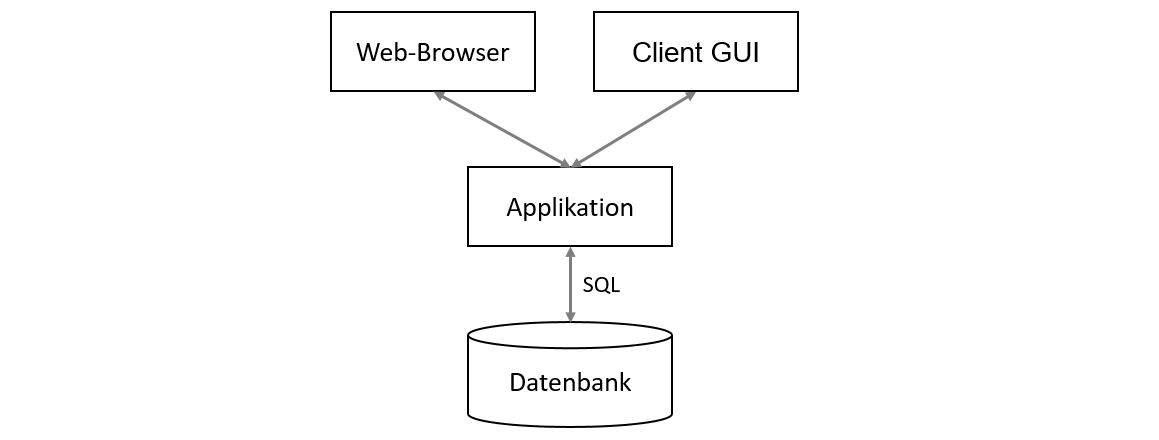
\includegraphics[width=\textwidth]{images/SQL_Injection/3TierArchitecture.jpg}
	\caption{3-Schichten-Architektur}
	\label{fig:3TierArchitecture}
\end{figure}

DBS werden von Endanwendern nicht direkt genutzt, sondern werden durch die Applikation und graphische Oberflächen verschalt. Der Benutzer greift z.B. via HTTP über die Oberfläche auf die Applikation zu. Die Applikation selbst ist mit einem dedizierten Datenbankbenutzer mit dem DBS verbunden, die Kommunikation erfolgt über SQL. Diese Architektur wird wegen ihrer drei Ebenen - der Präsentations-, der Logik- und der Persistenzschicht - auch als 3-Schichten-Architektur bezeichnet (vergleiche Abbildung \ref{fig:3TierArchitecture}). 

Die Applikationen stellen dem Benutzer Eingabefelder zur Verfügung, mittels derer die Benutzer Daten auslesen, verändern oder neu erzeugen können. Die Benutzereingaben werden zu bereits vorgefertigten SQL-Statements hinzugefügt und an das DBS gesendet. Das DBS verarbeitet das Statement und sendet eine Antwort an die Anwendung zurück.

\subsection{Der Angriff}
Bei einer SQL-Injection werden, wie der Name schon impliziert, (Teile von) SQL-Statements an die normalen Benutzereingaben angehängt, um somit die Logik und die Sicherheitsmechanismen der Applikation zu umgehen.

Der SQL-Interpreter des DBMS führt das ursprüngliche und die angehängten Statements aus. Mittels geschickter SQL-Injections können über harmlose Benutzerschnittstellen ganze Datenbanken gelöscht werden.

\section{Vorbereitung}
Für die Ausführung des Tutorials wird Kali Linux 2.0 mit eingerichteter Security Workbench benötigt. Alternativ kann das Skript auf einem anderen beliebigen Linux-System verwendet werden, in dem MySQL und Apache2 installiert sind. Zur korrekten Initialisierung der Webanwendung muss ggf. der Pfad zum Apache-Webserver in der Datei 'initializeDB.py' geändert werden. Die zu konfigurierenden Pfade im Quellcode sind entsprechend gekennzeichnet.

\section{Ablauf}
\subsection{Aufbau des Login-Web-Services}
Das Tutorial wird über die Security Workbench unter dem Hauptmenüpunkt 4 aufgerufen. Zu Beginn wird der Apache2-Webserver und das MySQL-DBMS gestartet. Anschließend wird die Datenbank initialisiert. Dabei wird folgendes Schema erstellt:
\begin{figure}[H]
	\centering
	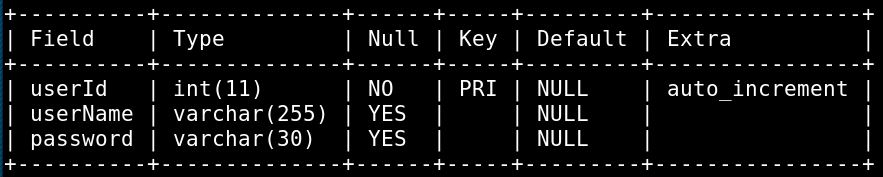
\includegraphics[width=\textwidth]{images/SQL_Injection/table_secretUserData.jpg}
	\caption{Tabellenstruktur der Tabelle \enquote{secretUserData}}
	\label{fig:table_secretUserData}
\end{figure}

Nun stehen verschiedene Tutorials zur Verfügung. Sie alle basieren auf demselben Web-Service, einem Login für eine Website (siehe Abbildung \ref{fig:user}). Der Web-Service wurde in HTML/CSS, JavaScript und PHP entwickelt. Die Benutzereingaben werden auf der HTML-Seite entgegen genommen und über einen Ajax-Aufruf an PHP übergeben. 

\begin{figure}[H]
	\centering
	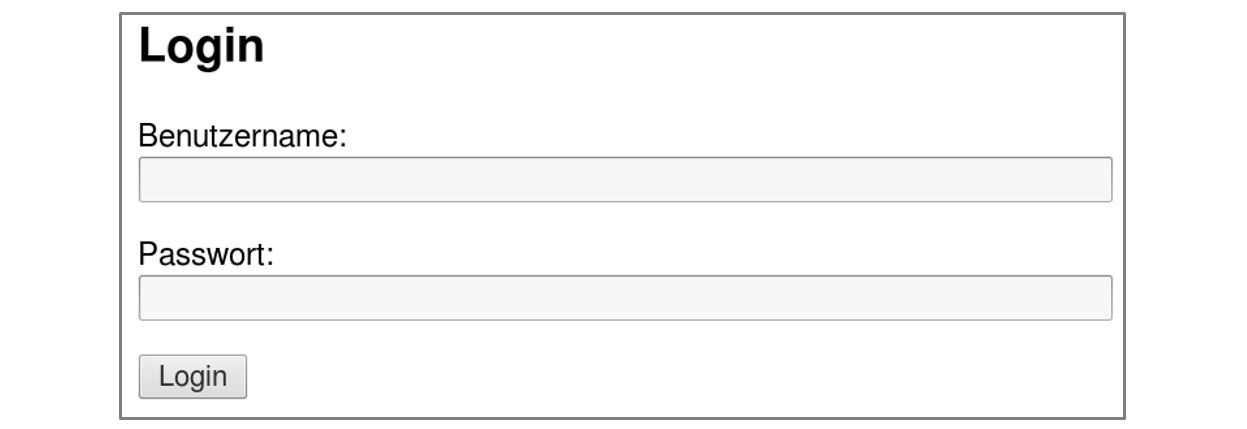
\includegraphics[width=\textwidth]{images/SQL_Injection/login.jpg}
	\caption{Login-Oberfläche des Web-Services}
	\label{fig:user}
\end{figure}

Dort werden die Benutzereingaben in ein vordefiniertes SQL-Statement eingefügt (siehe Listing \ref{lstlisting:SQL-Statement}) und an das DBS zur Ausführung übermittelt. Die Antwort des Servers, ein oder mehrere zutreffende Tupel mit der User-ID, dem User-Namen und dem User-Passwort werden anschließend unterhalb des Eingabefelds in dem Web-Service angezeigt. Dort ist ebenfalls das im DBS ausgeführte SQL-Statement zu sehen.

\begin{lstlisting}[caption=SQL-Statement\label{lstlisting:SQL-Statement}]{Name}
$query = '
	SELECT * 
	FROM secretUserData 
	WHERE userName = "'.$username.'" 
	AND   password = "'.$password.'";
';
\end{lstlisting}

Zudem sind zwei Buttons verfügbar, mit denen die Tabellenstruktur sowie der momentane Inhalt der Tabelle angezeigt werden können.

\subsection{SQL-Injection zum Auslesen von Daten}
Im ersten Teil des Tutorials werden mittels einer einfachen SQL-Injection Daten aus der Datenbank gelesen, auf die man über die Anwendung eigentlich keinen Zugriff hätte. Über die zwei Eingabefelder \enquote{Benutzername} und \enquote{Login} kann sich der Benutzer bei einer Anwendung anmelden. Die Eingaben werden an die Datenbank geschickt und in einem SELECT-Statement überprüft. Anschließend wird der selektierte Datensatz zurück geschickt.

Als erstes melden wir uns mit einem schon bekannten User und Passwort an, um die Funktionsweise zu testen. Nutze hierzu den User \colorbox{altgray}{\lstinline|Douglas Adams|} mit dem Passwort \colorbox{altgray}{\lstinline|DontPanic!|} und drücke auf den "Login"-Button."

\begin{figure}[H]
	\centering
	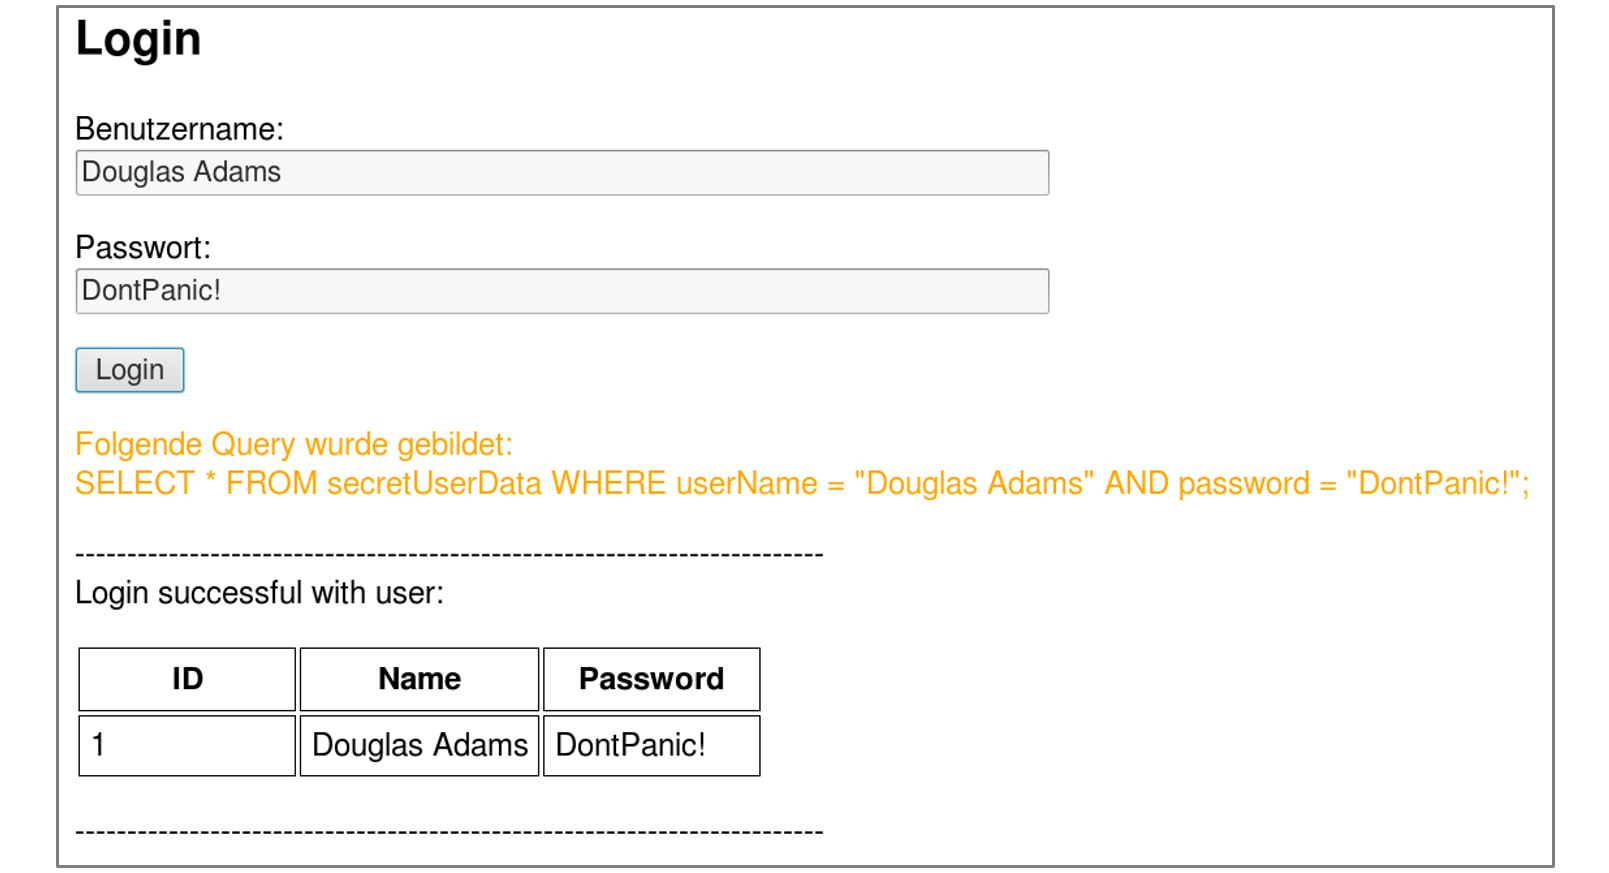
\includegraphics[width=\textwidth]{images/SQL_Injection/normal_login.jpg}
	\caption{Normaler Login}
	\label{fig:normal_login}
\end{figure}

Dieses Szenario spiegelt die angedachte Nutzung des Login-Dienstes wieder. Ein Nutzer meldet sich mit seinen Anmeldedaten an und deren Existenz wird in der Datenbank überprüft. Stimmen die Anmeldedaten überein, ist der Nutzer angemeldet und hat Zugriff auf die Anwendung.

Als nächstes sollen mittels einer SQL-Injection alle User der Datenbank \enquote{secretUserData} ausgegeben werden. Ersetze die aktuellen Eingaben hierzu z.B. durch \colorbox{altgray}{\lstinline|blabla" OR "1"="1|}. 

\begin{figure}[H]
	\centering
	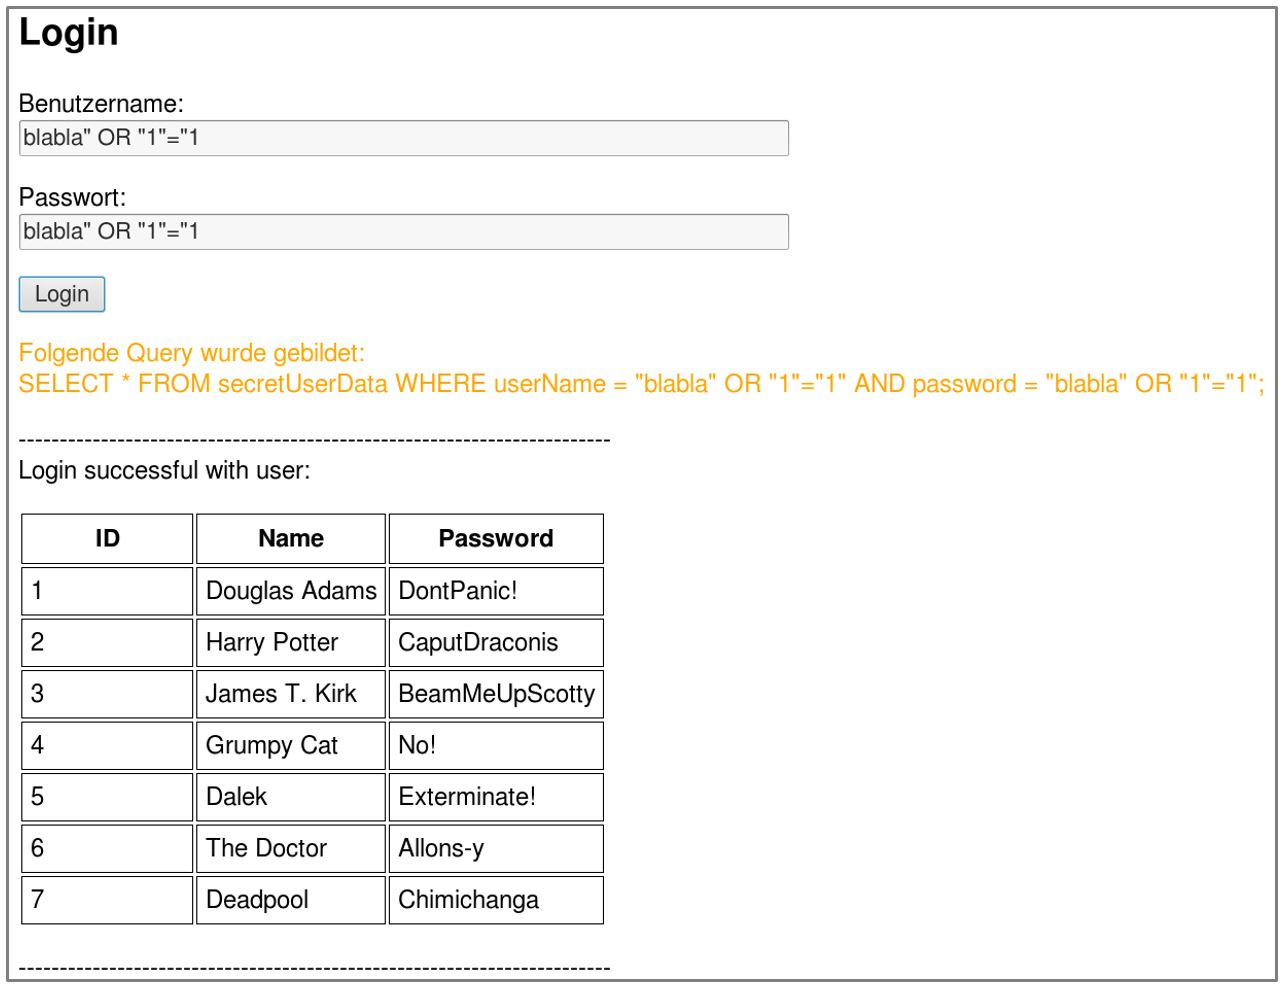
\includegraphics[width=\textwidth]{images/SQL_Injection/select_injection.jpg}
	\caption{Login mit SELECT-Injection}
	\label{fig:select_injection}
\end{figure}

Nun wurden alle Tupel, die in der Tabelle \enquote{secretUserData} enthalten sind ausgegeben. Möglich ist das durch das Anhängen von z.B. \colorbox{altgray}{\lstinline|OR "1"="1|} an eine beliebige Eingabe. Hierdurch werden die Abfragen der WHERE-Klausel grundsätzlich zu TRUE ausgewertet. Am obigen Beispiel erläutert bedeutet dies:
\begin{figure}[H]
	\centering
	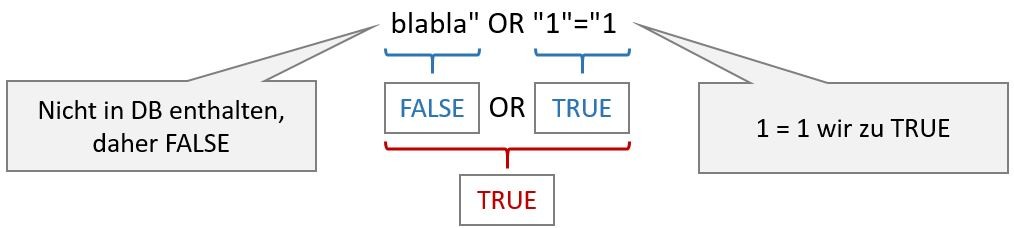
\includegraphics[width=\textwidth]{images/SQL_Injection/or1is1.jpg}
	\caption{Auswertung von OR "1"="1}
	\label{fig:or1is1}
\end{figure}
Sobald alle Ausdrücke innerhalb der WHERE-Klausel zu TRUE evaluiert wurden, wird die gesamte Datenbanktabelle ausgegeben. Hängt man den Zusatz lediglich an das Eingabefeld für das Passwort an, erhält man den Datensatz für den eingegebenen Benutzer. Dieses Szenario ist z.B. typisch, wenn man bereits einen möglichen Benutzernamen für die Applikation kennt, aber dessen Passwort unbekannt ist.

\subsection{SQL-Injection zum Einfügen von Daten}
Im zweiten Teil des Tutorials wird mittels einer SQL-Injection ein zusätzlicher Datensatz in die Tabelle eingefügt. Die Beispiel-Applikation ist äquivalent zu der aus dem ersten Tutorial. Dieses mal hängen wir an einen \colorbox{altgray}{\lstinline|beliebigen Benutzernamen|} folgendes INSERT-Statement inkl. Kommentar an: \shorthandoff{"}\colorbox{altgray}{\lstinline|"; INSERT INTO secretUserData VALUES(1234, "Hackerman", "fsociety"); --|}\shorthandon{"} . Im Eingabefeld für das Passwort können ebenfalls beliebige Zeichen eingegeben werden.
Durch diese Injection werden dem DBS prinzipiell drei Befehle übergeben:

\begin{figure}[H]
	\centering
	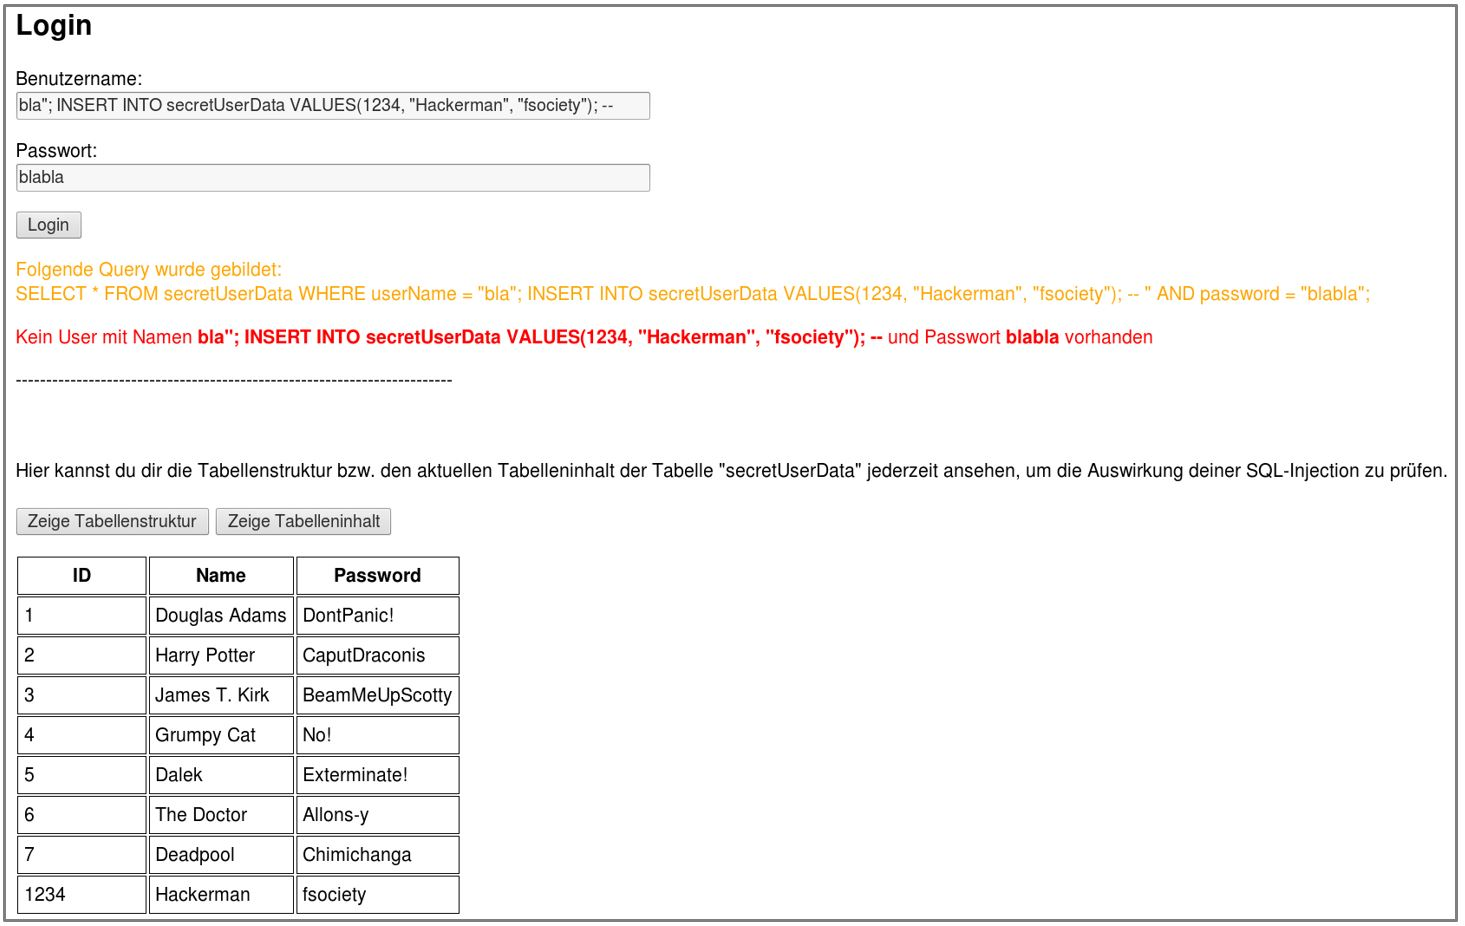
\includegraphics[width=\textwidth]{images/SQL_Injection/insert_injection.jpg}
	\caption{Login mit INSERT-Injection}
	\label{fig:insert_injection}
\end{figure}

\begin{itemize}
	\item Das ursprüngliche SELECT-Statement bis zur Eingabe eines Benutzers:  \colorbox{altgray}{\lstinline|SELECT * FROM secretUserData WHERE username = "<übergebener Benutzername>";|}
	\item Das angehängte INSERT-Statement:\\ \shorthandoff{"}\colorbox{altgray}{\lstinline|INSERT INTO secretUserData VALUES(1234, "Hackerman", "fsociety");|}\shorthandon{"}
	\item Ein Kommentar, der in SQL mit zwei Bindestrichen eingeleitet wird: \colorbox{altgray}{\lstinline|--|}. Hierdurch wird der SQL-Code, der noch zum ursprünglichen SELECT-Statement gehört, als Kommentar vom SQL-Interpreter ignoriert. Im Beispiel betrifft das: \shorthandoff{"}\colorbox{altgray}{\lstinline|" AND password = "<übergebenes Passwort>";|}\shorthandon{"}
\end{itemize}

Sieht man sich nach der Ausführung des Statements die Inhalte der Tabelle an, ist zu sehen, dass sich ein neuer Datensatz mit der User-ID 1234, dem Usernamen \enquote{Hackerman} und dem Passwort \enquote{fsociety} enthält. Nutzt man für die Injection zusätzlich einen existierenden Benutzernamen statt der Eingabe \enquote{bla}, wird man gleichzeitig bei der Applikation angemeldet.

\subsection{SQL-Injection zum Löschen von Tabellen}
Im dritten Teil des Tutorials wird mittels einer SQL-Injection die komplette Tabelle gelöscht (DROP).
 
Bitte beachte, dass du die Datenbank erst im Hauptmenü des Konsolen-Skripts im Unterpunkt \enquote{5. Datenbank zurück setzen} wieder initialisieren musst, wenn du nach dem DROP weiterarbeiten möchtest! 
 
Nun hängen wir an einen \colorbox{altgray}{\lstinline|beliebigen Benutzernamen|} folgendes Statement inkl. Kommentar an: \shorthandoff{"}\colorbox{altgray}{\lstinline|"; DROP TABLE secretUserData; --|}\shorthandon{"} . Im Eingabefeld für das Passwort können ebenfalls beliebige Zeichen eingegeben werden.
 
\begin{figure}[H]
	\centering
	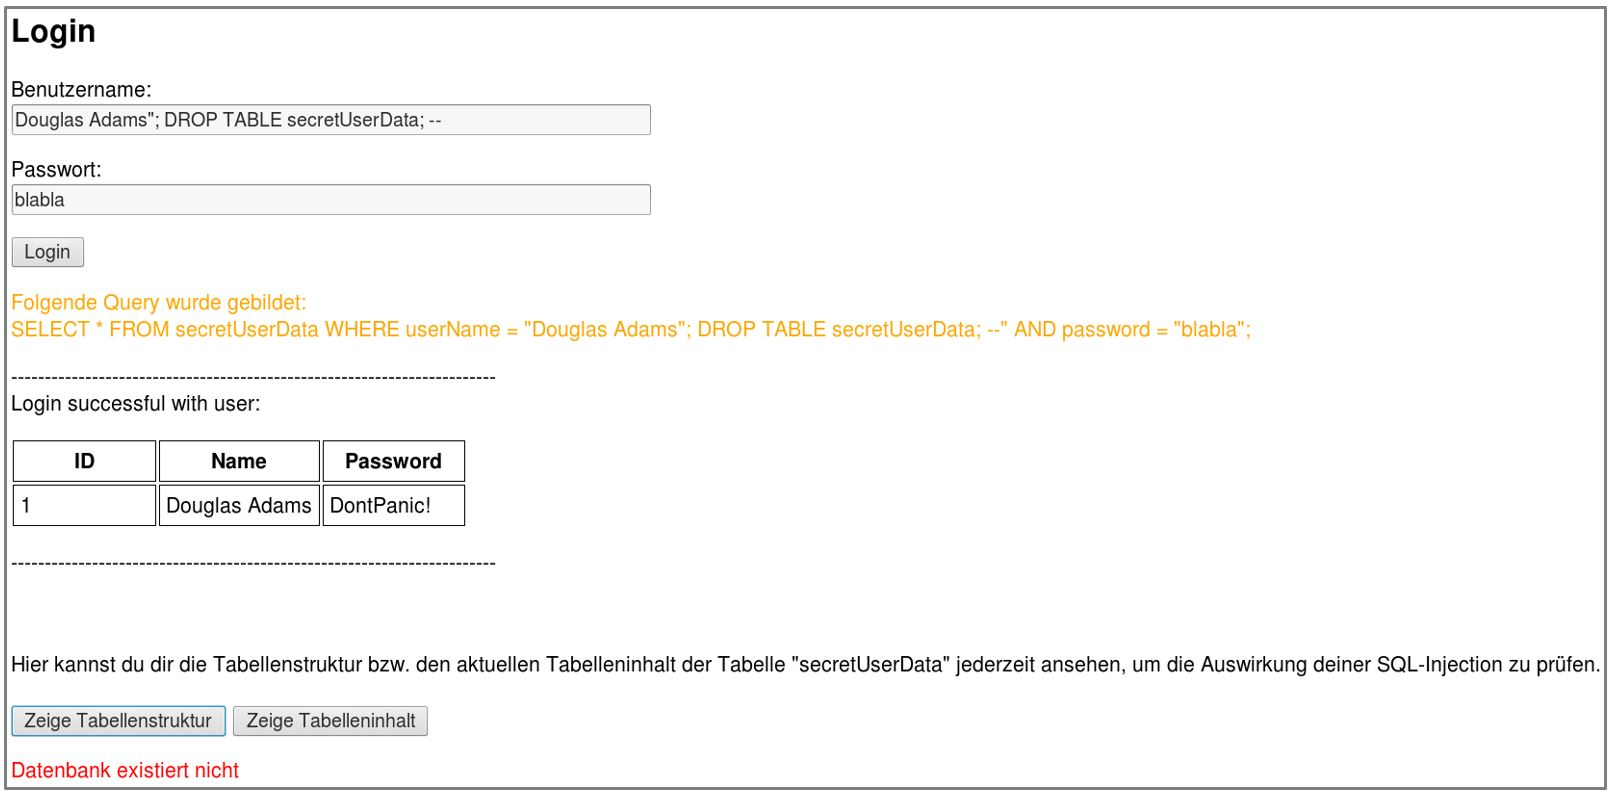
\includegraphics[width=\textwidth]{images/SQL_Injection/drop_injection.jpg}
	\caption{Login mit DROP-Injection}
	\label{fig:drop_injection}
\end{figure}

Die Ausführung der drei Statements (SELECT, DROP, Kommentar) ist äquivalent zum vorherigen Beispiel.

\subsection{SQL-Injection zum Modifizieren von Tabellen}
Das vierte Tutorial befasst sich mit modifizierenden SQL-Queries, die den Inhalt einer bestehenden Datenbanktabelle verändern. Technisch wird dies mit dem Update-Statement realisiert (siehe Listing \ref{lstlisting:SQL-UPDATE-Statement}).

\begin{lstlisting}[caption=SQL-UPDATE-Statement\label{lstlisting:SQL-UPDATE-Statement}]{Name}
$query = '
	UPDATE table_name
	SET column1 = value1, column2 = value2, ...
	WHERE condition; 
';
\end{lstlisting}
In Bezug auf das Tutorial umfasst die Datenbank eine Tabelle \colorbox{altgray}{\lstinline|sqlRanking|}, die eine virtuelle Rangliste entspricht (siehe Abbildung \ref{fig:sql-modify-ranking}). Diese besitzt die Spalten Username und Punkte. Zudem wird während der Initialisierung der Webseite die Rangliste auf Basis der Punktzahl absteigend sortiert.

\begin{figure}[H]
	\centering
	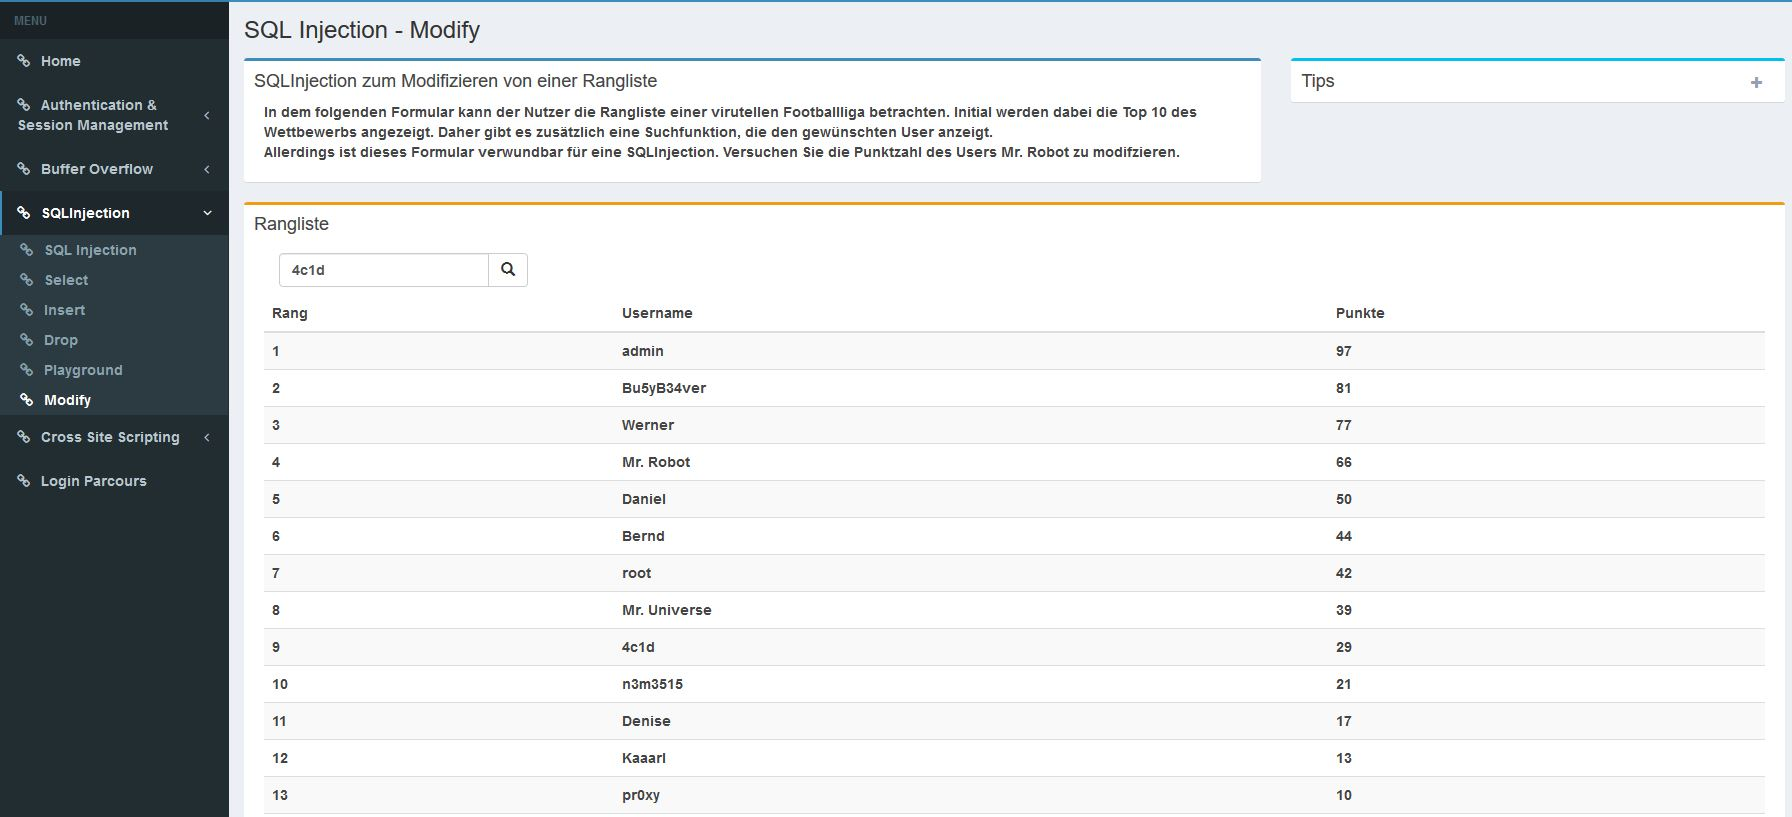
\includegraphics[width=\textwidth]{images/SQL_Injection/sql_modify.jpg}
	\caption{Rangliste mit Suchfunktion}
	\label{fig:sql-modify-ranking}
\end{figure}

Als Anwendungsszenario ist es hierbei möglich, die Rangliste mit einer Suchfunktion nach bestimmten Usernamen zu filtern. Abbildung \ref{fig:sql-modify-ranking-searched} zeigt wie der Anwender mit Hilfe des Input-Feldes nach einem gewünschten User sucht. Die Kommunikation mit der Datenbank basiert hierbei auf einem einfachen SELECT-Query.

\begin{figure}[H]
	\centering
	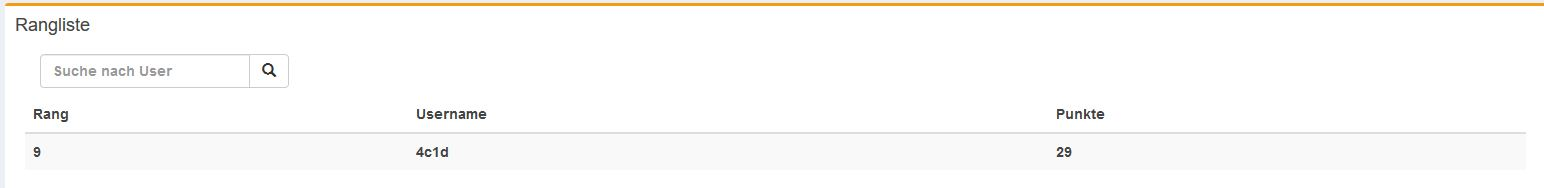
\includegraphics[width=\textwidth]{images/SQL_Injection/sql_modify_searched.jpg}
	\caption{Rangliste mit gesuchtem User}
	\label{fig:sql-modify-ranking-searched}
\end{figure}

An dieser Stelle gilt es hervorzuheben, dass die SQL-Abfrage nicht absichert ist und somit eine Sicherheitslücke entsteht. Im Folgenden ist das Ziel des Tutorials die Punkteanzahl eines Users zu modifizieren. 

Um die Aufgabe zu lösen, muss der Anwender in das Input-Feld ein SQL-Statement einfügen, das bspw. \\ \colorbox{altgray}{\lstinline|';  UPDATE sqlInjectionRanking SET punkte = 999 WHERE username = 'Mr. Robot|} entspricht. Wichtig ist das die erste SELECT-Abfrage gültig ist. Abbildung \ref{fig:sql-modify-ranking-solved} zeigt wie die Lösung des Tutorials aussehen kann. 

\begin{figure}[H]
	\centering
	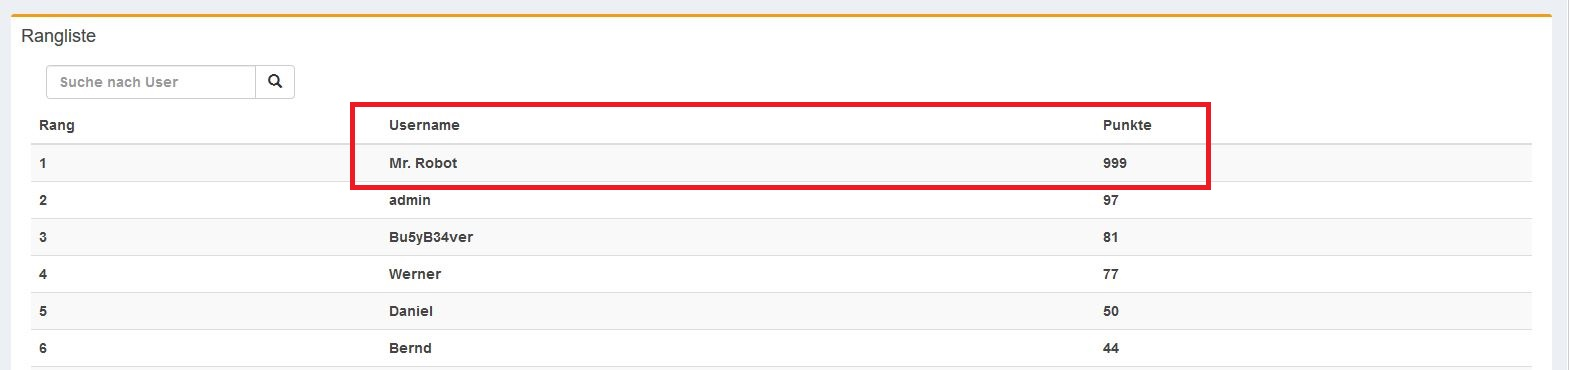
\includegraphics[width=\textwidth]{images/SQL_Injection/sql_modify_solved.jpg}
	\caption{Rangliste mit gesuchtem User}
	\label{fig:sql-modify-ranking-solved}
\end{figure}

Um das Tutorial zu vereinfachen, bekommt der Anwender je nach Wissensstand Tipps an die Hand, die ihn zur Lösung der Aufgabe hinführen sollen. 


\subsection{Die SQL-Injection-Spielwiese}
Im letzten Tutorial der SQL-Injection in der Broken-Web-Anwendung findest du die SQL-Injection-Spielwiese. Innerhalb dieser Spielwiese kannst du beliebige SQL-Injections ausprobieren.

\begin{figure}[H]
	\centering
	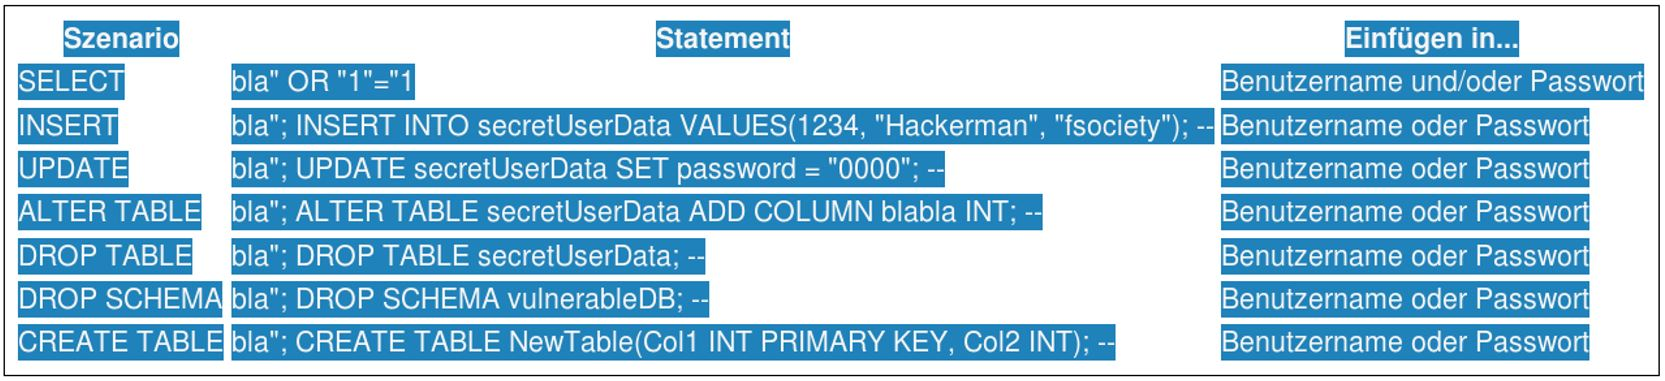
\includegraphics[width=\textwidth]{images/SQL_Injection/various_injections.jpg}
	\caption{Verschiedene SQL-Injections zum Ausprobieren}
	\label{fig:various_injections}
\end{figure}

Als Hinweis sind die Statements der vorhergegangenen Beispiele und einige Weitere im nachfolgenden Fenster hinterlegt. Um sie zu sehen musst du lediglich den Inhalt des Fensters mit der Maus markieren. Bitte beachte, dass du die Datenbank im Hauptmenü des Konsolen-Skripts im Unterpunkt \enquote{5. Datenbank zurück setzen} wieder initialisieren musst, wenn du nach einer Datenstruktur verändernden SQL-Injection weiter arbeiten willst. Dazu musst du die Anwendung nicht schließen. Deine Änderungen am Inhalt oder an der Struktur der Datenbank kannst du mit der Anzeige der Tabellenstruktur bzw. dem Inhalt jederzeit prüfen.\\

Neben den hier aufgelisteten gibt es noch eine Vielzahl weiterer SQL-Injections. Nicht alle werden in diesem Beispiel funktionieren, da der Erfolg von SQL-Injections von mehreren Faktoren abängig ist:
\begin{itemize}
	\item Die Programmiersprache der Anwendung
	\item Das verwendete DBMS
	\item Die Berechtigungen, die der Datenbankbenutzer der Anwendung inne hat
\end{itemize}

\section{Gegenmaßnahmen}
Viele Programmiersprachen haben mittlerweile Mechanismen eingebaut, mittels derer SQL-Injections abgewehrt werden können. So ist es in den meisten Programmier- und Skriptsprachen nicht mehr möglich, innerhalb eines DB-Aufrufs mehrere SQL-Statements auszuführen. In einigen wenigen ist dies immer noch möglich, wie z.B. in der Skriptsprache PHP.
\subsection{Prepared Statements}
Durch sogenannte \enquote{Prepared Statements} können SQL-Injections vollständig unterbunden werden. Statt das SQL-Statement komplett auf der Applikationsseite zusammenzustellen, wird das Statement auf zwei Mal an das DBS gesendet. Im ersten Aufruf wird das vorbereitete Statement ohne die Nutzereingaben an das DBS übermittelt. Hierdurch wird dem DBS die Struktur des Statements im Vorfeld angekündigt. Nachfolgend ist das Prepared Statement eines SELECT-Statements zu sehen:
\begin{lstlisting}[caption=Prepared Statement]{Name}
prepare("SELECT * FROM secretUserData where userName = ?");
\end{lstlisting}

Die vom Nutzer eingegebenen Parameter werden erst im Anschluss an das DBS übermittelt:
\begin{lstlisting}[caption=Übergabe der Parameter]{Name}
execute($_GET['name']);
\end{lstlisting}
Dort werden sie in das bereits angekündigte Statement eingefügt und ausgeführt. Übergebene Parameter, auch wenn ihnen SQL-Code hinzugefügt wurde, werden ausschließlich als Textinput interpretiert. 
\subsection{Escapen von Eingaben}
Eine weitere Möglichkeit die Datenbank vor unberechtigtem Zugriff und Manipulationen zu schützen ist das Escapen aller Nutzereingaben.
Das grundlegende Problem bei SQL-Injections ist die Interpretation von Texteingaben als ausführbare Anweisungen für das DBMS. Durch das Escapen der Eingaben werden Metazeichen wie Anführungszeichen maskiert und somit vom SQL-Interpreter nicht beachtet. Nachfolgend ist das Escapen von Strings in PHP dargestellt:
\begin{lstlisting}[caption=Escapen von Strings in PHP]{Name}
mysql_real_escape_string("some String");
\end{lstlisting}

%!TEX root = ../document.tex
\chapter{Disclaimer}
\label{ch:disclaimer}

Das vorliegende Dokument und das zugehörige Tool \enquote{Security Workbench} sind im Rahmen eines Projektes des Masterstudiengangs Informatik an der Technischen Hochschule Ingolstadt (THI) im Wintersemester 2016/17 entstanden. Sinn und Zweck der Security Workbench ist es, interessierten Studierenden das Thema IT-Security näher zu bringen. Alle hier gezeigten Tutorials sind ausschließlich für den Einsatz innerhalb einer eigens dafür geschaffenen Umgebung (z.B. dediziertes WLAN zum Durchspielen der Angriffsszenarien) mit der Zustimmung aller Beteiligten (sowohl Angreifer als auch Angegriffene) gedacht.

Der Missbrauch der zur Verfügung gestellten Informationen und Tutorials für kriminelle Handlungen kann strafrechtliche Folgen nach sich ziehen. Strafrechtliche Grundlagen sind hierbei u.a.:
\begin{itemize}
	\item§202a StGB – Ausspähen von Daten
	\item§202b StGB – Abfangen von Daten
	\item§202c StGB – Vorbereiten des Ausspähens und Abfangens von Daten
	\item§263 StGB – Computerbetrug
	\item§269 StGB – Fälschung beweiserheblicher Daten
	\item§270 StGB – Täuschung im Rechtsverkehr bei DV
	\item§§ 271, 274, 348 StGB – Falschbeurkundung/Urkundenunterdrückung im Zusammenhang mit DV
	\item§303a StGB – Datenveränderung
	\item§303b StGB – Computersabotage
\end{itemize}

Haftungsansprüche gegen die Autoren oder die THI im Falle der missbräuchlichen Verwendung der Informationen und des Tutorials sind ausgeschlossen. Die Autoren und die THI distanzieren sich ausdrücklich von der Verwendung der Informationen und des Tutorials für kriminelle Handlungen.

Die Autoren und die THI übernimmt keinerlei Gewähr für die Aktualität, Korrektheit, Vollständigkeit oder Qualität der bereitgestellten Informationen. Haftungsansprüche gegen die Autoren oder die THI, welche sich auf Schäden materieller oder ideeller Art beziehen, die durch die Nutzung oder Nichtnutzung der dargebotenen Informationen und Tutorials verursacht wurden, sind grundsätzlich ausgeschlossen. Die Autoren behalten es sich ausdrücklich vor, Teile der Dokumentation bzw. des Tutorials oder das gesamte Angebot ohne gesonderte Ankündigung zu verändern, zu ergänzen, zu löschen oder die Veröffentlichung zeitweise oder endgültig einzustellen.

Bei direkten oder indirekten Verweisen auf fremde Quellen und Internetseiten, die außerhalb des Verantwortungsbereichs der Autoren liegen, würde eine Haftungsverpflichtung ausschließlich in dem Fall in Kraft treten, in dem die Autoren von den Inhalten Kenntnis haben und es ihnen technisch möglich und zumutbar wäre, die Nutzung im Falle rechtswidriger Inhalte zu verhindern. Die Autoren erklären daher ausdrücklich, dass zum Zeitpunkt der Linksetzung die entsprechenden verlinkten Seiten frei von illegalen Inhalten waren. Die Autoren haben keinerlei Einfluss auf die aktuelle und zukünftige Gestaltung und auf die Inhalte der verknüpften Quellen und Seiten. Deshalb distanzieren sie sich hiermit ausdrücklich von allen Inhalten aller verknüpften Quellen und Seiten, die nach der Verknüpfung verändert wurden. Für illegale, fehlerhafte oder unvollständige Inhalte und insbesondere für Schäden, die aus der Nutzung oder Nichtnutzung solcherart dargebotener Informationen entstehen, haftet allein der Anbieter der Seite, auf welche verwiesen wurde, nicht derjenige, der über Links auf die jeweilige Veröffentlichung lediglich verweist.



%Ende Text
\end{document}